\documentclass[10pt,a4paper]{paper}

\usepackage[latin1]{inputenc}
\usepackage[english]{babel}

\usepackage[official,right]{eurosym}
\usepackage{hyperref}
\usepackage{graphicx}
\usepackage{a4wide}
\usepackage{calc}
%\usepackage{picins}
\usepackage{fancyhdr}
\usepackage{amssymb,amsmath}
\usepackage{gensymb}
%\usepackage{multicol}
\usepackage{url}

% For drawings
\usepackage{pgf}
\usepackage{tikz}
\usetikzlibrary{arrows,automata}
\usepackage{color}

% For quick and easy figures
\newcommand{\pic}[3]{
\begin{figure}[h]\begin{center}\includegraphics[width=#2]{#1.png} 
	\caption{#3}
	\label{#1}
\end{center}\end{figure}
}

\newcommand{\inHfile}[2]{
	Function \texttt{#1} in File \texttt{#2.h} \\
}

%\numberwithin{equation}{section}
\newcommand{\vect}[1]{\ensuremath{\overrightarrow{#1}}}		%% How to mark Vectors
\newcommand{\eu}[1]{\ensuremath{#1^{\phi}}}			%% how to mark euler angles
\newcommand{\ra}[1]{\ensuremath{\omega_{#1}}}		%% how to mark rates
\newcommand{\ew}[1]{\;. \! \!#1}					%% how to mark element-wise operations
\newcommand{\mat}[1]{\ensuremath{\mathbf{#1}}}		%% how to mark Matrices
\newcommand{\eye}[0]{\mat{I}}						%% Identity matrix
\newcommand{\quat}[1]{\ensuremath{q_{#1}}}			%% how to mark Quaternions
\newcommand{\transp}[1]{\ensuremath{#1^{T}}}
\newcommand{\est}[1]{\ensuremath{\hat{#1}}}
\newcommand{\err}[1]{\ensuremath{\tilde{#1}}}
\newcommand{\meas}[1]{\ensuremath{\tilde{#1}}}
\newcommand{\linpt}[1]{\ensuremath{\overline{#1}}}
\newcommand{\norm}[1]{\ensuremath{|{#1}|}}
\newcommand{\quatprod}[0]{\ensuremath{\bullet}}
\newcommand{\ddt}[2]{\ensuremath{#1^{(#2)}}}
\newcommand{\deriv}[2]{\ensuremath{{#1}^{(#2)}}}
\newcommand{\inv}[1]{\ensuremath{#1}^{-1}}
\newcommand{\comp}[1]{\ensuremath{#1}^*}
\newcommand{\atan}[1]{\ensuremath{\text{atan}\left({#1}\right)}}
\newcommand{\sign}[1]{\ensuremath{\text{sign}\left({#1}\right)}}
\newcommand{\cross}{\ensuremath{\times}}

\newcommand{\division}[0]{\ensuremath{\div}}
\newcommand{\multiplication}[0]{\ensuremath{\cdot}}


%% Formatting in the right color for euler angles
\definecolor{rollcolor}{rgb}{0,0,1}
\definecolor{pitchcolor}{rgb}{0,0.5,0}
\definecolor{yawcolor}{rgb}{1,0,0}
\newcommand{\Rollc}[1]{\color{rollcolor}#1\color{black}{}}
\newcommand{\Pitchc}[1]{\color{pitchcolor}#1\color{black}{}}
\newcommand{\Yawc}[1]{\color{yawcolor}#1\color{black}{}}
\newcommand{\Roll}[0]{\ensuremath{\Rollc \phi}}
\newcommand{\Pitch}[0]{\ensuremath{\Pitchc \theta }}
\newcommand{\Yaw}[0]{\ensuremath{\Yawc \psi}}


\newcommand{\mynote}[1]{\begin{flushright}\fbox{Martin: ``\textit{#1}''}\end{flushright}}
%\newcommand{\mynote}[1]{}

\graphicspath{{./images/},{tmp/}}

\title{Documentation for pprz_algebra}
\author{Martin Dieblich}

\begin{document}

%\maketitle
\section{Introduction}
This is the documentation for the algebra files of the paparazzi project (paparazzi.nongnu.org). It should be a reference for the functions which are defined in the directory \texttt{(paparazzi)/sw/airborne/math}. The structure of this documentation is in the way how it should make most sense in a mathematical content. This documentation might be redundant.\\
The Conversion between FLOAT and REAL to BFP(binary floating point)and vice versa is not in this documentation yet.

\section{Important definition} \label{Important definition}
Unfortunately there are a lot of different definitions for rotations. There are 24 (some say 12, the author tends to think that there are much more) different ways to define euler angles. Therefore, paparazzi uses the convention, which is shown in \textit{figure \ref{Normal euler order}}.
\begin{figure}[h!]\begin{center}
	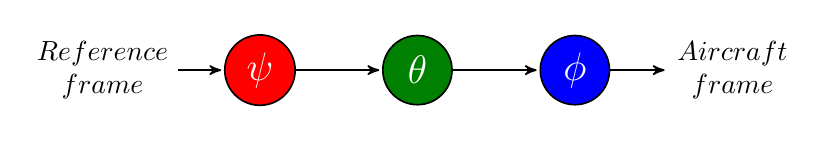
\begin{tikzpicture}[->,>=stealth',shorten >=1pt,auto,node distance=2cm,
                    semithick]
  \tikzstyle{every state}=[draw=black,text=white]

  \node		   (A)                    {$\begin{matrix}Reference\\frame\end{matrix}$};
  \node[state, fill=yawcolor]        (B) [right of=A] {\Large $\psi$};
  \node[state, fill=pitchcolor]         (C) [right of=B] {\Large $\theta$};
  \node[state, fill=rollcolor]         (D) [right of=C] {\Large $\phi$};
  \node         (E)		   [right of=D] {$\begin{matrix}Aircraft\\frame\end{matrix}$};

  \path (A) edge              node {} (B)
  		(B) edge              node {} (C)
  		(C) edge              node {} (D)
  		(D) edge              node {} (E);

	\end{tikzpicture}
	\caption{The order of rotation from the reference frame to the body frame is first \Yawc{Yaw}, then \Pitchc{Pitch} and finally \Rollc{Roll}.}
	\label{Normal euler order}
\end{center}\end{figure}
For instance, a resulting rotational matrix would be 
\begin{equation}
\mat R(\Yaw) \multiplication \mat R(\Pitch) \multiplication \mat R(\Roll)
\end{equation}
\begin{equation}
\begin{pmatrix}
cos(\Yaw) & -sin(\Yaw) & 0 \\
sin(\Yaw) &  cos(\Yaw) & 0 \\
0         &      0     & 1
\end{pmatrix} \multiplication \begin{pmatrix}
 cos(\Pitch) & 0 & sin(\Pitch) \\
 0         & 1 &     0     \\
-sin(\Pitch) & 0 & cos(\Pitch) 
\end{pmatrix} \multiplication \begin{pmatrix}
1 & 0         &     0      \\
0 & cos(\Roll) & -sin(\Roll) \\
0 & sin(\Roll) &  cos(\Roll) 
\end{pmatrix}
\end{equation}
\begin{equation}
\begin{pmatrix}
cos(\Pitch)cos(\Yaw)	& sin(\Roll)sin(\Pitch)cos(\Yaw) - cos(\Roll)cos(\Yaw)	& cos(\Roll)sin(\Pitch)cos(\Yaw) + sin(\Roll)sin(\Yaw)\\
cos(\Pitch)sin(\Yaw)	& sin(\Roll)sin(\Pitch)sin(\Yaw) + cos(\Roll)cos(\Yaw)	& cos(\Roll)sin(\Pitch)sin(\Yaw) - sin(\Roll)cos(\Yaw) \\
-sin(\Pitch)			& sin(\Roll)cos(\Pitch)									& cos(\Roll)cos(\Pitch)
\end{pmatrix}
\end{equation}

An equivalent multiplication from a quaternion with a vector would be
\begin{equation}
\begin{pmatrix}0\\\vect v_o\end{pmatrix} = \quat{} \quatprod \begin{pmatrix}0\\\vect v_i\end{pmatrix} \quatprod \comp{\quat{}}
\end{equation}


But, since paparazzi is a library for aerospace, the \emph{choosen perspective is from the vehicle}. This is an important difference, because the attitude representation changes slightly, but it can mess up everything. In detail this means, that the order of the euler angles changes and also the sign\footnote{If you have problems understanding this, pages 123f and 130-134 of [1] help a lot!}(figure \ref{Aerospace euler order}).
\mynote{I still need to fix the citation}
\begin{figure}[h]\begin{center}
	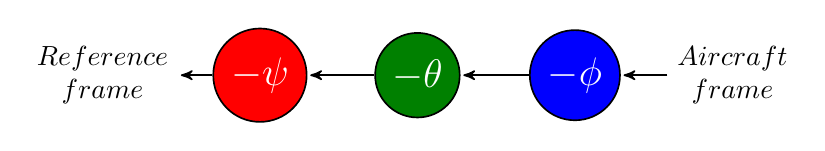
\begin{tikzpicture}[->,>=stealth',shorten >=1pt,auto,node distance=2cm,
                    semithick]
  \tikzstyle{every state}=[draw=black,text=white]

  \node		   (A)                    {$\begin{matrix}Reference\\frame\end{matrix}$};
  \node[state, fill=yawcolor]        (B) [right of=A] {\Large $-\psi$};
  \node[state, fill=pitchcolor]         (C) [right of=B] {\Large $-\theta$};
  \node[state, fill=rollcolor]         (D) [right of=C] {\Large $-\phi$};
  \node         (E)		   [right of=D] {$\begin{matrix}Aircraft\\frame\end{matrix}$};

  \path (C) edge              node {} (B)
  		(D) edge              node {} (C)
  		(E) edge              node {} (D)
  		(B) edge              node {} (A);

	\end{tikzpicture}
	\caption{From the perspective of the vehicle the order and the sign of the euler angles change.}
	\label{Aerospace euler order}
\end{center}\end{figure}
As a result the rotational matrix changes to the transposed/inverted.
\begin{equation} \label{order of matrix multiplication}
\mat R(-\Roll) \multiplication \mat R(-\Pitch) \multiplication \mat R(-\Yaw)
\end{equation}
\begin{equation}
\begin{pmatrix}
cos(\Pitch)cos(\Yaw)									& cos(\Pitch)sin(\Yaw)									& -sin(\Pitch)			\\
sin(\Roll)sin(\Pitch)cos(\Yaw) - cos(\Roll)cos(\Yaw)	& sin(\Roll)sin(\Pitch)sin(\Yaw) + cos(\Roll)cos(\Yaw)	& sin(\Roll)cos(\Pitch)	\\
cos(\Roll)sin(\Pitch)cos(\Yaw) + sin(\Roll)sin(\Yaw)	& cos(\Roll)sin(\Pitch)sin(\Yaw) - sin(\Roll)cos(\Yaw)	& cos(\Roll)cos(\Pitch)
\end{pmatrix}
\end{equation}
Same for the quaternion multiplication
\begin{equation}
\begin{pmatrix}0\\\vect v_o\end{pmatrix} = \comp{\quat{}} \quatprod \begin{pmatrix}0\\\vect v_i\end{pmatrix} \quatprod \quat{}
\end{equation}

\section{Overview}
An Overview of the implemented functions\\
\newcommand{\YES}{$\surd$}
\newcommand{\NO}{}
\begin{tabular}{c|ccccccc}
function	& VECT2	& VECT3	& MAT33	& RMAT	& EULER	& RATES	& QUAT	\\  \hline
ZERO		& \YES	& \YES	& \NO	& \NO	& \NO	& \NO	& \NO	\\
ASSIGN		& \YES	& \YES	&(\YES) &(\YES) & \YES	& \YES	& \YES	\\
COPY		& \YES	& \YES	& \YES	& \YES	& \YES	& \YES	& \YES	\\
ADD			& \YES	& \YES	& \NO	& \NO	& \YES	& \YES	& \YES	\\
SUM			& \YES	& \YES	& \NO	& \NO	& \NO	& \YES	& \NO	\\
SUB			& \YES	& \YES	& \NO	& \YES	& \YES	& \YES	& \NO	\\
DIFF		& \YES	& \YES	& \NO	& \NO	& \YES	& \YES	& \YES	\\
SMUL		& \YES	& \YES	& \NO	& \NO	& \YES	& \YES	& \YES	\\
EW\_MUL		& \NO	& \YES	& \NO	& \NO	& \NO	& \YES	& \NO	\\
SDIV		& \YES	& \YES	& \NO	& \NO	& \YES	& \YES	& \NO	\\
EW\_DIV		& \NO	& \YES	& \NO	& \NO	& \NO	& \NO	& \NO	\\
NORM		& \YES	& \YES	& \NO	& \YES	& \YES	& \YES	& \YES	\\
STRIM		& \YES	& \YES	& \NO	& \NO	& \NO	& \NO	& \NO	\\
BOUND\_CUBE	& \NO	& \YES	& \NO	& \NO	& \YES	& \YES	& \NO	\\
BOUND\_BOX	& \NO	& \YES	& \NO	& \NO	& \NO	& \YES	& \NO
\end{tabular}
\mynote{Add Compiler \#warning or \#error for wrong use of Bound and Strim?}
\tableofcontents
\section{Scalar}
For scalar values are a few functions available

\subsection{Multiplication and Rightshift}
Represents $ a \multiplication b $ with a right shift about \textit{r}. This becomes close to
\begin{equation}
2^{-r} a \multiplication b
\end{equation}
but it is not the same.
\inHfile{INT\_MULT\_RSHIFT(a, b, r)}{pprz\_algebra\_int}

\subsection{$\sqrt x$ Squareroot}
Calculates the squareroot $y = \sqrt x$. The function uses the Babylonian method.
\begin{equation}
y_{n+1} = \frac 1 2 \left( y_n + \frac{x}{y_n} \right)
\end{equation}
\inHfile{INT32\_SQRT(out,in)}{pprz\_algebra\_int}

\subsection{atan2() 4-quadrant arctangent}
Calculates the 4-quadrant arctangent of two values, x and y:
\begin{equation}
a = atan2(y,x)
\end{equation}
The function uses a trick, which is desribed in detail at
\begin{itemize}
\item http://www.dspguru.com/comp.dsp/tricks/alg/fxdatan2.htm
\end{itemize}
In short:


\begin{figure}[h!]
	\centering
	\begin{tabular}{ccc}
	
		\begin{minipage}{4cm}
		\centering
		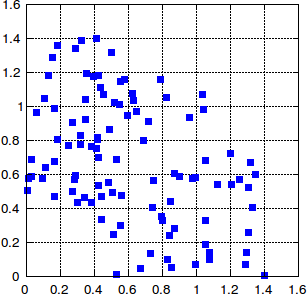
\includegraphics[width=4cm]{xyvalues}
		\end{minipage}
	&
		\begin{minipage}{4cm}
		\centering
		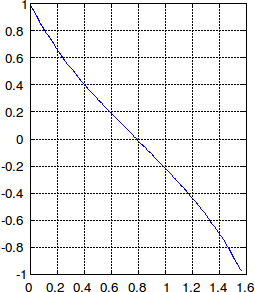
\includegraphics[width=4cm]{ratiofunction}
		\end{minipage}
	&
		\begin{minipage}{5cm}
		\centering
		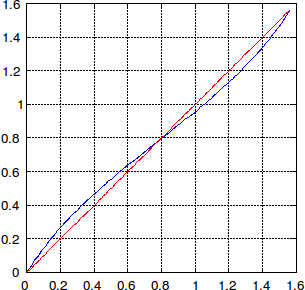
\includegraphics[width=4cm]{atan2_alternate}
		\end{minipage}
	\\
		(a) x/y-values  &
		(b) ratio function & 
		(c) comparison of the result (blue)
	\\
		& & and the real value (red)
	\end{tabular}
	
	\caption{alternate atan2 function} \label{alternate atan2 function}
\end{figure}

If you have a set of x/y values (figure \ref{alternate atan2 function}a), you can compute the ratio (figure \ref{alternate atan2 function}b) of them:
\begin{equation}
	r = \frac{x+y}{x-y}
\end{equation}
and transform this ratio very close to the real values (figure \ref{alternate atan2 function}c) using
\begin{equation}
	\alpha = \tfrac \pi 4 (1-r)
\end{equation}
or (more accurate) using
\begin{equation}
	\alpha_2 = 0.1963 \multiplication r^3 -0.9817 \multiplication r + \tfrac \pi 4
\end{equation}
\inHfile{INT32\_ATAN2(a, y, x)}{pprz\_algebra\_int}
\inHfile{INT32\_ATAN2\_2(a, y, x)}{pprz\_algebra\_int}
\section{Vector}
\subsection{Definition}
The main definition for every vector struct is that the values are called x, y and z (if it's a 3D-vector):
\begin{equation}
\vect v = \begin{pmatrix}x\\y\end{pmatrix} \quad oor \quad \vect v = \begin{pmatrix}x\\y\\z\end{pmatrix}
\end{equation}
It is available for the following simple types:\\
\begin{tabular}{c|c|c}
type		& struct 2D		& struct 3D\\ \hline
uint16\_t	& 				& Uint16Vect3	\\
int16\_t 	& 				& Int16Vect3	\\
int32\_t	& Int32Vect2	& Int32Vect3	\\
int64\_t	& Int32Vect2	& Int32Vect3	\\
float		& FloatVect2	& FloatVect3	\\
double		& DoubleVect2	& DoubleVect3	
\end{tabular}


\subsection{= Assigning}
\subsubsection*{$\vect{v} = \vect{0}$}
\begin{equation}
 \vect v = \begin{pmatrix} 0 \\ 0 \end{pmatrix} \qquad or \qquad  \vect v = \begin{pmatrix} 0 \\ 0 \\ 0 \end{pmatrix}
\end{equation}
\inHfile{INT\_VECT2\_ZERO(v)}{pprz\_algebra\_int}
\inHfile{INT\_VECT3\_ZERO(v)}{pprz\_algebra\_int}
\inHfile{INT32\_VECT3\_ZERO(v)}{pprz\_algebra\_int}
\inHfile{FLOAT\_VECT2\_ZERO(v)}{pprz\_algebra\_float}
\inHfile{FLOAT\_VECT3\_ZERO(v)}{pprz\_algebra\_float}

\subsubsection*{$\vect{a} = \transp{(x,y)}$ or $\vect a = \transp{(x,y,z)}$}
\begin{equation}
 \vect a = \begin{pmatrix} x \\ y \end{pmatrix} \qquad or \qquad  \vect a = \begin{pmatrix} x \\ y \\ z \end{pmatrix}
\end{equation}
\inHfile{VECT2\_ASSIGN(a, x, y)}{pprz\_algebra}
\inHfile{VECT3\_ASSIGN(a, x, y, z)}{pprz\_algebra}
\inHfile{FLOAT\_VECT2\_ASSIGN(a, x, y)}{pprz\_algebra\_float}
\inHfile{FLOAT\_VECT3\_ASSIGN(a,x,y,z)}{pprz\_algebra\_float}


\subsubsection*{$\vect{a} = \vect{b}$}
\begin{equation}
\vect a = \vect b
\end{equation}
\inHfile{VECT2\_COPY(a, b)}{pprz\_algebra}
\inHfile{VECT3\_COPY(a, b)}{pprz\_algebra}
\inHfile{INT32\_VECT3\_COPY(o, i)}{pprz\_algebra\_int}
\inHfile{FLOAT\_VECT2\_COPY(a, b)}{pprz\_algebra\_float}




\subsection{+ Addition}
\subsubsection*{$\vect{a} += \vect{b}$}
\begin{equation}
\vect a = \vect a + \vect b
\end{equation}
\inHfile{VECT2\_ADD(a, b)}{pprz\_algebra}
\inHfile{VECT3\_ADD(a, b)}{pprz\_algebra}
\inHfile{INT32\_VECT3\_ADD(a, b)}{pprz\_algebra\_int}
\inHfile{FLOAT\_VECT2\_ADD(a, b)}{pprz\_algebra\_float}


\subsubsection*{$\vect{c} = \vect{a} + \vect{b}$}
\begin{equation}
\vect c = \vect a + \vect b
\end{equation}
\inHfile{VECT2\_SUM(c, a, b)}{pprz\_algebra}
\inHfile{VECT3\_SUM(c, a, b)}{pprz\_algebra}
\inHfile{INT32\_VECT3\_SUM(c, a, b)}{pprz\_algebra\_int}
\inHfile{FLOAT\_VECT2\_SUM(c, a, b)}{pprz\_algebra\_float}
\inHfile{DOUBLE\_VECT3\_SUM(c, a, b)}{pprz\_algebra\_double}



\subsection{- Subtraction}
\subsubsection*{$\vect{a} -= \vect{b}$}
\begin{equation}
\vect a = \vect a - \vect b
\end{equation}
\inHfile{VECT2\_SUB(a, b)}{pprz\_algebra}
\inHfile{VECT3\_SUB(a, b)}{pprz\_algebra}
\mynote{no INT32 vect3 sub?}
\inHfile{FLOAT\_VECT2\_SUB(a, b)}{pprz\_algebra\_float}
\inHfile{FLOAT\_VECT3\_SUB(a, b)}{pprz\_algebra\_float}

\subsubsection*{$\vect{c} = \vect{a} - \vect{b}$}
\begin{equation}
\vect c = \vect a - \vect b
\end{equation}
\inHfile{VECT2\_DIFF(c, a, b}{pprz\_algebra}
\inHfile{VECT3\_DIFF(c, a, b)}{pprz\_algebra}
\inHfile{INT32\_VECT3\_DIFF(c, a, b)}{pprz\_algebra\_int}
\inHfile{FLOAT\_VECT2\_DIFF(c, a, b)}{pprz\_algebra\_float}
\inHfile{FLOAT\_VECT3\_DIFF(c, a, b)}{pprz\_algebra\_float}






\subsection{$\multiplication$ Multiplication}
\subsubsection*{$\vect{v_o} = s \multiplication \vect{v_i}$ With a scalar}
\begin{equation}
	\vect{v_o} = s \multiplication \vect{v_i}
\end{equation}
\inHfile{VECT2\_SMUL(vo, vi, s)}{pprz\_algebra}
\inHfile{VECT3\_SMUL(vo, vi, s)}{pprz\_algebra}
\inHfile{FLOAT\_VECT2\_SMUL(vo, vi, s)}{pprz\_algebra\_float}
\inHfile{FLOAT\_VECT3\_SMUL(vo, vi, s)}{pprz\_algebra\_float}
or with a fraction
\begin{equation}
	\vect{a} = \frac{num}{den} \multiplication \vect{b}
\end{equation}
\inHfile{INT32\_VECT2\_SCALE\_2(a, b, num, den)}{pprz\_algebra\_int}
\inHfile{INT32\_VECT3\_SCALE\_2(a, b, num, den)}{pprz\_algebra\_int}

\subsubsection*{$\vect{v_o} = \vect{v_a} \ew\multiplication \vect{v_b} $ Element-wise}
Also known as the ``Dot-Multiplication'' from MATLAB, Octave or FreeMat.
\begin{equation}
	\begin{pmatrix}x_o\\y_o\\z_o\end{pmatrix} = 
	\begin{pmatrix}x_a \multiplication x_b\\y_a \multiplication y_b\\z_a \multiplication z_b\end{pmatrix}
\end{equation}
\inHfile{VECT3\_EW\_MUL(vo, va, vb)}{pprz\_algebra}
\mynote{Nothing for VECT2?}

\subsubsection*{$\vect v_o = \vect v_1 \cross \vect v_2$ Cross-Product}
\begin{equation}
\vect v_o = \vect v_1 \cross \vect v_2 = \begin{pmatrix}
 0   & -z_1 &  y_1 \\
 z_1 &  0   & -x_1 \\
-y_1 &  x_1 &  0
\end{pmatrix} \multiplication \begin{pmatrix}x_2\\y_2\\z_2\end{pmatrix}
\end{equation}
\inHfile{FLOAT\_VECT3\_CROSS\_PRODUCT(vo, v1, v2)}{pprz\_algebra\_float}
\inHfile{DOUBLE\_VECT3\_CROSS\_PRODUCT(vo, v1, v2)}{pprz\_algebra\_double}

\subsubsection*{$\vect v_{out} = \mat{A} \multiplication \vect v_{in}$ With a Matrix}
\begin{equation}
\vect v_{out} = \mat A \multiplication \vect v_{in}
\end{equation}
\inHfile{MAT33\_VECT3\_MUL(vout, mat, vin)}{pprz\_algebra}
\inHfile{RMAT\_VECT3\_MUL(vout, rmat, vin)}{pprz\_algebra}
\inHfile{FLOAT\_RMAT\_VECT3\_MUL(vout, rmat, vin)}{pprz\_algebra\_float}
\inHfile{DOUBLE\_MAT33\_VECT3\_MUL(vout, mat, vin)}{pprz\_algebra\_double}
\begin{equation}
\vect v_{out} = \transp{\mat A} \multiplication \vect v_{in}
\end{equation}
\inHfile{MAT33\_VECT3\_TRANSP\_MUL(vout, mat, vin)}{pprz\_algebra}
\inHfile{DOUBLE\_MAT33\_VECT3\_TRANSP\_MUL(vout, mat, vin)}{pprz\_algebra\_double}
For rotational matrices, with additional right shift about the decimal point position:
\begin{equation}
\vect v_b = \mat M_{a2b} \multiplication \vect v_a
\end{equation}
\inHfile{INT32\_RMAT\_VMULT(vb, m\_a2b, va)}{pprz\_algebra\_int}
With the transposed matrix
\begin{equation}
\vect v_b = \transp{\mat M_{b2a}} \multiplication \vect v_a
\end{equation}
\inHfile{INT32\_RMAT\_TRANSP\_VMULT(vb, m\_b2a, va)}{pprz\_algebra\_int}

With choosable right-shift:
\begin{equation}
\vect v_{out} = 2^{-f} \mat M \multiplication \vect v
\end{equation}
\inHfile{INT32\_MAT33\_VECT3\_MULT(o, m, v, f)}{pprz\_algebra\_int}

\subsubsection*{$\vect v_{out} = \quat{} \quatprod \vect v_{in}$ With a quaternion}
The quaternion is transformed to a rotational matrix and then the vector is multiplied with the matrix
\begin{equation}
\vect v_{out} = \quat{} \quatprod \vect v_{in}
\end{equation}
\begin{equation}
\vect v_{out} = \mat R_m(\quat{}) \multiplication \vect v_{in}
\end{equation}
\begin{equation}
\vect v_{out} = \begin{pmatrix}
1-2(q_y + q_z)		& 2(q_xq_y-q_iq_z)	& 2(q_xq_z + q_iq_y) \\
2(q_xq_y + q_iq_z)	& 1-2(q_x + q_z)	& 2(q_yq_z - q_iq_x) \\
2(q_xq_z - q_iq_y)	& 2(q_yq_z+q_iq_x)	& 1-2(q_x + q_y)	
\end{pmatrix}
 \multiplication \vect v_{in}
\end{equation}
\inHfile{INT32\_QUAT\_VMULT(v\_out, q, v\_in)}{pprz\_algebra\_int}
\inHfile{FLOAT\_QUAT\_VMULT(v\_out, q, v\_in)}{pprz\_algebra\_float}



\subsection{$\division$ Division}
\subsubsection*{$\vect{v_o} = \frac 1 s \multiplication \vect{v_i}$ With a scalar}
\begin{equation}
	\vect{v_o} = \frac 1 s \multiplication \vect{v_i}
\end{equation}
\inHfile{VECT2\_SDIV(vo, vi, s)}{pprz\_algebra}
\inHfile{VECT3\_SDIV(vo, vi, s)}{pprz\_algebra}
\inHfile{INT32\_VECT3\_SDIV(a, b, s)}{pprz\_algebra\_int}

\subsubsection*{$\vect{v_o} = \vect{v_a} \ew\division \vect{v_b} $ Element-wise}
Also known as the ``Dot-Division'' from MATLAB, Octave or FreeMat.
\begin{equation}
	\begin{pmatrix}x_o\\y_o\\z_o\end{pmatrix} = 
	\begin{pmatrix}x_a \division x_b\\y_a \division y_b\\z_a \division z_b\end{pmatrix}
\end{equation}
\inHfile{VECT3\_EW\_DIV(vo, va, vb)}{pprz\_algebra}
\mynote{Nothing for VECT2?}





\subsection{Other}
\subsubsection*{$\norm{\vect{v}}$ Norm}
Computes the 2-norm of a vector (the length).
\begin{equation}
n = \norm{\vect{v}} = \sqrt{\vect v \multiplication \vect v} = \sqrt{x \multiplication x + y \multiplication y} \quad or \quad \sqrt{x \multiplication x + y \multiplication y + z \multiplication z}
\end{equation}
\inHfile{INT32\_VECT2\_NORM(n, v)}{pprz\_algebra\_int}
\inHfile{INT32\_VECT3\_NORM(n, v)}{pprz\_algebra\_int}
\inHfile{FLOAT\_VECT3\_NORM(v)}{pprz\_algebra\_float}
\mynote{float differs from int!}
Alternatively you can normalize a 3D - vector directly using
\inHfile{FLOAT\_VECT3\_NORMALIZE(v)}{pprz\_algebra\_float}

\subsubsection*{Right-Shift}
Makes an bitwise right-shift with every value. This is close to the multiplication with $ 2^{-r} $, but not the same.
\begin{equation}
\vect v_o = 2^{-r} \vect v_i
\end{equation}
\inHfile{INT32\_VECT2\_RSHIFT(o, i, r)}{pprz\_algebra\_int}

\subsubsection*{Left-Shift}
Makes an bitwise left-shift with every value. This is close to the multiplication with $ 2^{l} $, but not the same.
\begin{equation}
\vect v_o = 2^{l} \vect v_i
\end{equation}
\inHfile{INT32\_VECT2\_LSHIFT(o, i, l)}{pprz\_algebra\_int}

\subsubsection*{$min \leq \vect v \leq max$ Bounding}
Bounds the vector so that every value is between \textit{min} and \textit{max}.
\begin{eqnarray}
\vect v \in \mathbb{I}^2 \qquad or \qquad \vect v \in \mathbb{I}^3, \\
\mathbb{I} = [min; max]
\end{eqnarray}
\textbf{WARNING:}\\
The functions ``\texttt{STRIM}'' have a higher priority for the lower border. So, if $ min > max$ and a value of $ \vect v $ is between those, the value is set to min. \\
The function ``\texttt{BOUND\_CUBE}'' does that the other way round.\\
\inHfile{VECT2\_STRIM(v, min, max)}{pprz\_algebra}
\inHfile{VECT3\_STRIM(v, min, max)}{pprz\_algebra}
\inHfile{VECT3\_BOUND\_CUBE(v, min, max)}{pprz\_algebra}
\mynote{VECT3\_STRIM and VECT3\_BOUND\_CUBE do nearly the same.}

\subsubsection*{$\vect{v}_{min} \leq \vect v \leq \vect{v}_{max}$ Bounding}
Ensures that
\begin{equation}
\vect v_{min} \leq \vect v \leq \vect v_{max} \Leftrightarrow \begin{pmatrix} x_{min} \\ y_{min} \\ z_{min} \end{pmatrix} \leq \begin{pmatrix} x \\ y \\ z \end{pmatrix} \leq \begin{pmatrix} x_{max} \\ y_{max} \\ z_{max} \end{pmatrix}
\end{equation}
\inHfile{VECT3\_BOUND\_BOX(v, v\_min, v\_max}{pprz\_algebra}
\mynote{Nothing for VECT2?}

\subsubsection*{Rounding}
Rounds the values of a double vector to integer values.
\begin{equation}
\vect v_{out} = rint(\vect v_{in})
\end{equation}
\inHfile{DOUBLE\_VECT3\_RINT(vout, vin)}{pprz\_algebra\_double}
\section{Matrix $3\times3$ / Rotation Matrix}
The indices of a matrix are zero-indexed, i.e. the first element in the matrix has the row and column number \textbf{Zero}.
\mynote{I choosed to start the indices with 1.}
\subsection{Definition}
The matrix is represented as an array with the length 9.
\begin{equation}
\mat M = \begin{pmatrix}
m_0 & m_1 & m_2 \\
m_3 & m_4 & m_5 \\
m_6 & m_7 & m_8
\end{pmatrix} = \begin{pmatrix}
m[0] & m[1] & m[2] \\
m[3] & m[4] & m[5] \\
m[6] & m[7] & m[8]
\end{pmatrix}
\end{equation}
It is available for the following simple types:\\
\begin{tabular}{c|c|c}
type		& struct Mat	& struct RMat	\\ \hline
int32\_t	& Int32Mat33	& Int32RMat		\\
float		& FloatMat33	& FloatRMat		\\
double		& DoubleMat33	& DoubleRMat
\end{tabular}



\subsection{= Assigning}
\subsubsection*{$\mat M = \mat 0$}
\begin{equation}
\mat M = \begin{pmatrix}
0 & 0 & 0 \\
0 & 0 & 0 \\
0 & 0 & 0
\end{pmatrix}
\end{equation}
\inHfile{FLOAT\_MAT33\_ZERO(m)}{pprz\_algebra\_float}
\inHfile{FLOAT\_RMAT\_ZERO(m)}{pprz\_algebra\_float}

\subsubsection*{$a_{ij}$ elements}
Accessing an element is able with
\inHfile{MAT33\_ELMT(m, row, col)}{pprz\_algebra}
\inHfile{RMAT\_ELMT(m, row, col)}{pprz\_algebra}

\subsubsection*{$\mat M = diag(d_{00}, d_{11}, d_{22})$}
\begin{equation}
\mat M = \begin{pmatrix}
d_{00} & 0 & 0 \\
0 & d_{11} & 0 \\
0 & 0 & d_{22}
\end{pmatrix}
\end{equation}
\inHfile{FLOAT\_MAT33\_DIAG(m, d00, d11, d22)}{pprz\_algebra\_float}

\subsubsection*{$\mat{A} = \mat{B}$}
\begin{equation}
\mat {mat1} = \mat {mat2}
\end{equation}
\inHfile{MAT33\_COPY(mat1, mat2)}{pprz\_algebra}
\inHfile{RMAT\_COPY(o, i)}{pprz\_algebra}


\subsubsection*{$\mat M_{b2a} = \inv{\mat M_{a2b}} = \transp{\mat M_{a2b}}$}
\begin{equation}
\mat M_{b2a} = \inv{\mat M_{a2b}} = \transp{\mat M_{a2b}}
\end{equation}
\inHfile{FLOAT\_RMAT\_INV(m\_b2a, m\_a2b)}{pprz\_algebra\_float}

\subsection{- Subtraction}
\subsubsection*{$\mat C = \mat A - \mat B$}
\begin{equation}
\mat C = \mat A - \mat B
\end{equation}
\inHfile{RMAT\_DIFF(c, a, b)}{pprz\_algebra}
For bigger matrices you have to spezify the number of rows (\texttt{i}) and the number of columns (\texttt{j}).
\inHfile{MAT\_SUB(i, j, C, A, B)}{pprz\_simple\_matrix}



\subsection{$\multiplication$ Multiplication}
\subsubsection*{$\mat M_{a2c} = \mat M_{b2c} \multiplication \mat M_{a2b}$ with a Matrix (composition)}
Makes a matrix-multiplication with additional Right-Shift about the decimal point.
\mynote{Not quite sure about that}
\begin{equation}
\mat M_{a2c} = \mat M_{b2c} \multiplication \mat M_{a2b}
\end{equation}
\inHfile{INT32\_RMAT\_COMP(m\_a2c, m\_a2b, m\_b2c)}{pprz\_algebra\_int}
\inHfile{FLOAT\_RMAT\_COMP(m\_a2c, m\_a2b, m\_b2c)}{pprz\_algebra\_float}
and with the inverse matrix
\begin{equation}
\mat M_{a2b} = \inv{\mat M_{b2c}} \multiplication \mat M_{a2c}
\end{equation}
\inHfile{INT32\_RMAT\_COMP\_INV(m\_a2b, m\_a2c, m\_b2c)}{pprz\_algebra\_int}
\inHfile{FLOAT\_RMAT\_COMP\_INV(m\_a2b, m\_a2c, m\_b2c)}{pprz\_algebra\_float}
Multiplication is also possible with bigger matrices
\begin{equation}
\mat C_{i \cross j} = \mat A_{i \cross k} \multiplication \transp{\mat B_{j \cross k}}
\end{equation}
\inHfile{MAT\_MUL\_T(i, k, j, C, A, B)}{pprz\_simple\_matrix}
or
\begin{equation}
\mat C_{i \cross j} = \mat A_{i \cross k} \multiplication \mat B_{k \cross j}
\end{equation}
\inHfile{MAT\_MUL(i, k, j, C, A, B)}{pprz\_simple\_matrix}


\subsection{Transformation from a Matrix}
\subsubsection*{to euler angles}
\mynote{This is only for the 321-convention}
The rotation matrix from euler angles is known
\begin{equation}
\mat R_m = \begin{pmatrix}
cos(\Pitch)cos(\Yaw)									& cos(\Pitch)sin(\Yaw)									& -sin(\Pitch)			\\
sin(\Roll)sin(\Pitch)cos(\Yaw) - cos(\Roll)cos(\Yaw)	& sin(\Roll)sin(\Pitch)sin(\Yaw) + cos(\Roll)cos(\Yaw)	& sin(\Roll)cos(\Pitch)	\\
cos(\Roll)sin(\Pitch)cos(\Yaw) + sin(\Roll)sin(\Yaw)	& cos(\Roll)sin(\Pitch)sin(\Yaw) - sin(\Roll)cos(\Yaw)	& cos(\Roll)cos(\Pitch)
\end{pmatrix}
\end{equation}
and the extraction is done vice versa.
\begin{equation}
\eu e = \begin{pmatrix}\Roll \\ \Pitch \\ \Yaw \end{pmatrix} = 
\begin{pmatrix}
\arctan2(r_{23}, r_{33}) \\
-\arcsin(r_{13}) \\
\arctan2(r_{12}, r_{11})
\end{pmatrix}
\end{equation}
\inHfile{INT32\_EULERS\_OF\_RMAT(e, rm)}{pprz\_algebra\_int}
\inHfile{FLOAT\_EULERS\_OF\_RMAT(e, rm)}{pprz\_algebra\_float}


\subsubsection*{to a quaternion}
Since the construction of a matrix from a quaternion is known
\begin{equation}
\mat R_m = \begin{pmatrix}
1-2(q_y^2 + q_z^2)		& 2(q_xq_y-q_iq_z)		& 2(q_xq_z + q_iq_y) \\
2(q_xq_y + q_iq_z)		& 1-2(q_x^2 + q_z^2)	& 2(q_yq_z - q_iq_x) \\
2(q_xq_z - q_iq_y)		& 2(q_yq_z+q_iq_x)		& 1-2(q_x^2 + q_y^2)	
\end{pmatrix},
\end{equation}
the extraction of a quaternion is done vice versa. But there are obviously many opportunities to extract the quaternion. They differ in the way which element of the quaternion is extracted from the diaognal elements $r_{11}$, $r_{22}$ and $r_{33}$  of the matrix.
\begin{equation}
1 = q_i^2+q_x^2+q_y^2+q_z^2
\end{equation}
\textbf{First case}
\begin{eqnarray}
\zeta = \sqrt{1 + (r_{11}+r_{22}+r_{33})}  =  \sqrt{1 + (3q_i^2 -q_x^2 -q_y^2 -q_z^2)} = \sqrt{4 q_i^2} \\
q_i = \tfrac 1 2 \zeta \\
q_x =  \tfrac 1 {2 \zeta} (r_{23}-r_{32}) \\
q_y =  \tfrac 1 {2 \zeta} (r_{31}-r_{13}) \\
q_z =  \tfrac 1 {2 \zeta} (r_{12}-r_{21})
\end{eqnarray}
\textbf{Second case}
\begin{eqnarray}
\zeta = \sqrt{1 + (r_{11}-r_{22}-r_{33})}  =  \sqrt{1 + (-q_i^2+3q_x^2 -q_y^2 -q_z^2)} = \sqrt{4 q_x^2} \\
q_i =  \tfrac 1 {2 \zeta} (r_{23}-r_{32}) \\
q_x = \tfrac 1 2 \zeta \\
q_y =  \tfrac 1 {2 \zeta} (r_{12}+r_{21}) \\
q_z =  \tfrac 1 {2 \zeta} (r_{31}+r_{13})
\end{eqnarray}
\textbf{Third case}
\begin{eqnarray}
\zeta = \sqrt{1 + (-r_{11}+r_{22}-r_{33})}  =  \sqrt{1 + (-q_i^2 -q_x^2+3q_y^2 -q_z^2)} = \sqrt{4 q_y^2} \\
q_i =  \tfrac 1 {2 \zeta} (r_{31}-r_{13}) \\
q_x =  \tfrac 1 {2 \zeta} (r_{12}+r_{21}) \\
q_y = \tfrac 1 2 \zeta \\
q_z =  \tfrac 1 {2 \zeta} (r_{23}+r_{32})
\end{eqnarray}
\textbf{Fourth case}
\begin{eqnarray}
\zeta = \sqrt{1 + (-r_{11}-r_{22}+r_{33})}  =  \sqrt{1 + (-q_i^2 -q_x^2 -q_y^2+3q_z^2)} = \sqrt{4 q_z^2} \\
q_i =  \tfrac 1 {2 \zeta} (r_{12}-r_{21}) \\
q_x =  \tfrac 1 {2 \zeta} (r_{31}+r_{13}) \\
q_y =  \tfrac 1 {2 \zeta} (r_{23}+r_{32}) \\
q_z = \tfrac 1 2 \zeta
\end{eqnarray}
All are mathematicaly equivalent but numerically different. To avoid complex numbers and singularities the case with the biggest $\zeta$ should be choosen. 
\inHfile{INT32\_QUAT\_OF\_RMAT(q, r)}{pprz\_algebra\_int}
\inHfile{FLOAT\_QUAT\_OF\_RMAT(q, r)}{pprz\_algebra\_float}



\subsection{Tranformation to a Matrix}
\subsubsection*{from an axis and an angle}
With a known axis of rotation $\vect u$ and an angle $\alpha$ it is possible to compute a rotational matrix with
\begin{equation}
\mat R_m = \begin{pmatrix}
0 & -u_z & u_y \\
u_z & 0 & -u_x \\
-u_y & u_x & 0
\end{pmatrix} \sin \alpha + \left( \eye - \vect u \transp{\vect u} \right)\cos \alpha +  \vect u \transp{\vect u}.
\end{equation}
Please note again, that all angles are from the perspective of the aircraft (see section \ref{Important definition}). Therefore the angle is defined ngeative, leading to
\begin{equation}
\mat R_m = \begin{pmatrix}
0 & u_z & -u_y \\
-u_z & 0 & u_x \\
u_y & -u_x & 0
\end{pmatrix} \sin \alpha + \left( \eye - \vect u \transp{\vect u} \right)\cos \alpha +  \vect u \transp{\vect u}.
\end{equation}
Rearranging this equation leads to
\begin{equation}
\mat R_m = \begin{pmatrix}
u_x^2+(1-u_x^2)\cos \alpha				& u_xu_y(1-\cos \alpha) + u_z \sin \alpha	& u_xu_z(1-\cos \alpha) - u_y \sin \alpha \\
u_xu_y(1-\cos \alpha) - u_z \sin \alpha	& u_y^2+(1-u_y^2)\cos \alpha				& u_yu_z(1-\cos \alpha) + u_x \sin \alpha \\
u_xu_z(1-\cos \alpha) + u_y \sin \alpha & u_yu_z(1-\cos \alpha) - u_x \sin \alpha	& u_z^2+(1-u_z^2)\cos \alpha
\end{pmatrix}.
\end{equation}
\inHfile{FLOAT\_RMAT\_OF\_AXIS\_ANGLE(rm, uv, an)}{pprz\_algebra\_float}

\subsubsection*{from euler angles}
The transformation from euler angles $ \eu e$ to a rotational matrix depends on the order of rotation. Here, the default order is 321, which means first \Yawc{Yaw} (about the \emph{third} axis), then \Pitchc{Pitch} (the \emph{second} axis) and finally \Rollc{Roll}(the \emph{first} axis). Please note the important definition about perspectives (page \ref{Important definition}).
\begin{equation}
\mat R_m = \begin{pmatrix}
cos(\Pitch)cos(\Yaw)									& cos(\Pitch)sin(\Yaw)									& -sin(\Pitch)			\\
sin(\Roll)sin(\Pitch)cos(\Yaw) - cos(\Roll)cos(\Yaw)	& sin(\Roll)sin(\Pitch)sin(\Yaw) + cos(\Roll)cos(\Yaw)	& sin(\Roll)cos(\Pitch)	\\
cos(\Roll)sin(\Pitch)cos(\Yaw) + sin(\Roll)sin(\Yaw)	& cos(\Roll)sin(\Pitch)sin(\Yaw) - sin(\Roll)cos(\Yaw)	& cos(\Roll)cos(\Pitch)
\end{pmatrix}\end{equation}

\inHfile{INT32\_RMAT\_OF\_EULERS(rm, e)}{pprz\_algebra\_int}
\inHfile{INT32\_RMAT\_OF\_EULERS\_321(rm, e)}{pprz\_algebra\_int}
\inHfile{FLOAT\_RMAT\_OF\_EULERS(rm, e)}{pprz\_algebra\_float}
\inHfile{FLOAT\_RMAT\_OF\_EULERS\_321(rm, e)}{pprz\_algebra\_float}
You can also choose the 312 definition (First \Yawc{Yaw}, then  \Rollc{Roll} then \Pitchc{Pitch} $\Rightarrow \mat R(\Yaw) \mat R(\Roll)  \mat R(\Pitch)$). Again, remember the different order and sign:
\begin{equation}
\mat R_m = \mat R(-\Pitch) \mat R(-\Roll)  \mat R(-\Yaw)
\end{equation}
\begin{equation}
\mat R_m = \begin{pmatrix}
cos(\Pitch)cos(\Yaw)-sin(\Roll)sin(\Pitch)sin(\Yaw)		& cos(\Pitch)sin(\Yaw) + sin(\Roll)sin(\Pitch)cos(\Yaw)	& -cos(\Roll)sin(\Pitch) \\
-cos(\Roll)sin(\Yaw)									& cos(\Roll)cos(\Yaw)									& sin(\Roll)		\\
sin(\Pitch)cos(\Yaw) + sin(\Roll)cos(\Pitch)sin(\Yaw)	& sin(\Pitch)sin(\Yaw)-sin(\Roll)cos(\Pitch)cos(\Yaw)	& cos(\Roll)cos(\Pitch)
\end{pmatrix}\end{equation}
\inHfile{INT32\_RMAT\_OF\_EULERS\_312(rm, e)}{pprz\_algebra\_int}
\inHfile{FLOAT\_RMAT\_OF\_EULERS\_312(rm, e)}{pprz\_algebra\_float}
\inHfile{DOUBLE\_RMAT\_OF\_EULERS\_312(rm, e)}{pprz\_algebra\_float}


\subsubsection*{from a quaternion}
The most common definition for this transformation is
\begin{equation}
\mat R_m = \begin{pmatrix}
1-2(q_y^2 + q_z^2)		& 2(q_xq_y-q_iq_z)		& 2(q_xq_z + q_iq_y) \\
2(q_xq_y + q_iq_z)		& 1-2(q_x^2 + q_z^2)	& 2(q_yq_z - q_iq_x) \\
2(q_xq_z - q_iq_y)		& 2(q_yq_z+q_iq_x)		& 1-2(q_x^2 + q_y^2)	
\end{pmatrix}.
\end{equation}

\inHfile{INT32\_RMAT\_OF\_QUAT(rm, q)}{pprz\_algebra\_int}
\inHfile{FLOAT\_RMAT\_OF\_QUAT(rm, q)}{pprz\_algebra\_float}
\mynote{I called the quicker function "INT32\_RMAT\_OF\_QUAT\_QUICKER"}





\subsection{Other}
\subsubsection*{Trace}
\begin{equation}
tr(\mat{R}_m) = a_{11} + a_{22} + a_{33}
\end{equation}
\inHfile{RMAT\_TRACE(rm)}{pprz\_algebra}

\subsubsection*{$\norm{\norm{\mat M}}_F$ Norm (Frobenius)}
Calculates the Frobenius Norm of a matrix
\begin{equation}
\norm{\norm{\mat M}}_F = \sqrt{\sum_{i=1}^3 \sum_{i=1}^3 m_{ij}^2 }
\end{equation}
\inHfile{FLOAT\_RMAT\_NORM(m)}{pprz\_algebra\_float}

\subsection*{$\inv{\mat A} $ Inversion}
The inversion of a 3-by-3 matrix is made using the adjugate matrix and the determinant:
\begin{equation}
\inv{\mat A} = \frac{adj(\mat A)}{det(\mat A} = \frac{1}{det{\mat A}} \begin{pmatrix}
a_{22}a_{33}-a_{23}a_{32}&a_{13}a_{32}-a_{12}a_{33}&a_{12}a_{23}-a_{13}a_{22}\\
a_{23}a_{31}-a_{21}a_{33}&a_{11}a_{33}-a_{13}a_{31}&a_{13}a_{21}-a_{11}a_{23}\\
a_{21}a_{31}-a_{22}a_{31}&a_{12}a_{31}-a_{11}a_{32}&a_{11}a_{22}-a_{12}a_{21}
\end{pmatrix}
\end{equation}
\inHfile{MAT\_INV33(invS, S)}{pprz\_simple\_matrix}
\section{Euler Angles}
\subsection{Definition}
The values are called
\begin{equation}
\eu{e} = \begin{pmatrix} \Roll \\\Pitch\\\Yaw\\\end{pmatrix} = \begin{pmatrix} phi \\Pitch\\Yaw\\\end{pmatrix}
\end{equation}
It is available for the following simple types:\\
\begin{tabular}{c|c}
type		& struct		\\ \hline
int16\_t	& Int16Eulers	\\
int32\_t	& Int32Eulers	\\
float		& FloatEulers	\\
double		& DoubleEulers
\end{tabular}
\textbf{IMPORTANT:}\label{paparazzi euler definition}\\
Because there are many definitions of euler angles (some say 12, wikipedia says 24, the author tends to believe there are 48) and the choice of perspective, paparazzi choosed the following convention:




\subsection{= Assigning}
\subsubsection*{$\eu{e} = \eu{0}$}
\begin{equation}
\eu v = \begin{pmatrix} 0 \\ 0 \\ 0 \end{pmatrix}
\end{equation}
\inHfile{INT\_EULERS\_ZERO(e)}{pprz\_algebra\_int}
\inHfile{FLOAT\_EULERS\_ZERO(e)}{pprz\_algebra\_float}

\subsubsection*{$\eu a = \transp{(\Roll,\Pitch,\Yaw)}$}
\begin{equation}
\eu a = \transp{(\Roll,\Pitch,\Yaw)}
\end{equation}
\inHfile{EULERS\_ASSIGN(e, phi, theta, psi)}{pprz\_algebra}

\subsubsection*{$\eu a = \eu b$}
\begin{equation}
\eu a = \eu b
\end{equation}
\inHfile{EULERS\_COPY(a, b)}{pprz\_algebra}



\subsection{+ Addition}
\subsubsection*{$\eu a += \eu b$}
\begin{equation}
\eu a = \eu a + \eu b
\end{equation}
\inHfile{EULERS\_ADD(a, b)}{pprz\_algebra}
\mynote{No EULERS\_SUM function?}



\subsection{- Subtraction}
\subsubsection*{$\eu a -= \eu b$}
\begin{equation}
\eu a = \eu a - \eu b
\end{equation}
\inHfile{EULERS\_SUB(a, b)}{pprz\_algebra}

\subsubsection*{$\eu c = \eu a - \eu b$}
\begin{equation}
\eu c = \eu a - \eu b
\end{equation}
\inHfile{EULERS\_DIFF(c, a, b)}{pprz\_algebra}




\subsection{$\multiplication$ Multiplication}
\subsubsection*{$\eu{e_o} = s \multiplication \eu{e_i}$ With a scalar}
\begin{equation}
\eu e_o = s \multiplication \eu{e_i}
\end{equation}
\inHfile{EULERS\_SMUL(eo, ei, s)}{pprz\_algebra}




\subsection{$\division$ Division}
\subsubsection*{$\eu{e_o} = \frac 1 s \multiplication \eu{e_i}$ With a scalar}
\begin{equation}
\eu{e_o} = \frac 1 s \multiplication \eu{e_i}
\end{equation}
\inHfile{EULERS\_SDIV(eo, ei, s)}{pprz\_algebra}



\subsection{Transformation from euler angles}
\subsubsection*{to a rotational matrix}
The transformation from euler angles $ \eu e$ to a rotational matrix depends on the order of rotation. Here, the default order is 321, which means first \Yawc{Yaw} (about the \emph{third} axis), then \Pitchc{Pitch} (the \emph{second} axis) and finally \Rollc{Roll}(the \emph{first} axis). Please note the important definition about perspectives (page \ref{Important definition}).
\begin{equation}
\mat R_m = \begin{pmatrix}
cos(\Pitch)cos(\Yaw)									& cos(\Pitch)sin(\Yaw)									& -sin(\Pitch)			\\
sin(\Roll)sin(\Pitch)cos(\Yaw) - cos(\Roll)cos(\Yaw)	& sin(\Roll)sin(\Pitch)sin(\Yaw) + cos(\Roll)cos(\Yaw)	& sin(\Roll)cos(\Pitch)	\\
cos(\Roll)sin(\Pitch)cos(\Yaw) + sin(\Roll)sin(\Yaw)	& cos(\Roll)sin(\Pitch)sin(\Yaw) - sin(\Roll)cos(\Yaw)	& cos(\Roll)cos(\Pitch)
\end{pmatrix}\end{equation}

\inHfile{INT32\_RMAT\_OF\_EULERS(rm, e)}{pprz\_algebra\_int}
\inHfile{INT32\_RMAT\_OF\_EULERS\_321(rm, e)}{pprz\_algebra\_int}
\inHfile{FLOAT\_RMAT\_OF\_EULERS(rm, e)}{pprz\_algebra\_float}
\inHfile{FLOAT\_RMAT\_OF\_EULERS\_321(rm, e)}{pprz\_algebra\_float}
You can also choose the 312 definition (First \Yawc{Yaw}, then  \Rollc{Roll} then \Pitchc{Pitch} $\Rightarrow \mat R(\Yaw) \mat R(\Roll)  \mat R(\Pitch)$). Again, remember the different order and sign:
\begin{equation}
\mat R_m = \mat R(-\Pitch) \mat R(-\Roll)  \mat R(-\Yaw)
\end{equation}
\begin{equation}
\mat R_m = \begin{pmatrix}
cos(\Pitch)cos(\Yaw)-sin(\Roll)sin(\Pitch)sin(\Yaw)		& cos(\Pitch)sin(\Yaw) + sin(\Roll)sin(\Pitch)cos(\Yaw)	& -cos(\Roll)sin(\Pitch) \\
-cos(\Roll)sin(\Yaw)									& cos(\Roll)cos(\Yaw)									& sin(\Roll)		\\
sin(\Pitch)cos(\Yaw) + sin(\Roll)cos(\Pitch)sin(\Yaw)	& sin(\Pitch)sin(\Yaw)-sin(\Roll)cos(\Pitch)cos(\Yaw)	& cos(\Roll)cos(\Pitch)
\end{pmatrix}\end{equation}
\inHfile{INT32\_RMAT\_OF\_EULERS\_312(rm, e)}{pprz\_algebra\_int}
\inHfile{FLOAT\_RMAT\_OF\_EULERS\_312(rm, e)}{pprz\_algebra\_float}
\inHfile{DOUBLE\_RMAT\_OF\_EULERS\_312(rm, e)}{pprz\_algebra\_float}


\subsubsection*{to a quaternion}
The transformation is given by
\begin{equation}
\quat{} = [\cos \tfrac{\Yaw}{2} + \mathbf{k} \sin \tfrac{\Yaw}{2}][\cos \tfrac{\Pitch}{2} + \mathbf{j} \sin \tfrac{\Pitch}{2}][\cos \tfrac{\Roll}{2} + \mathbf{i} \sin \tfrac{\Roll}{2}]
\end{equation}
In matrix notation:
\begin{equation}
\quat = \begin{pmatrix}
\cos \tfrac{\Roll}{2} \cos \tfrac{\Pitch}{2} \cos \tfrac{\Yaw}{2} + \sin \tfrac{\Roll}{2} \sin \tfrac{\Pitch}{2} \sin \tfrac{\Yaw}{2} \\
\sin \tfrac{\Roll}{2} \cos \tfrac{\Pitch}{2} \cos \tfrac{\Yaw}{2} - \cos \tfrac{\Roll}{2} \sin \tfrac{\Pitch}{2} \sin \tfrac{\Yaw}{2} \\
\cos \tfrac{\Roll}{2} \sin \tfrac{\Pitch}{2} \cos \tfrac{\Yaw}{2} + \sin \tfrac{\Roll}{2} \cos \tfrac{\Pitch}{2} \sin \tfrac{\Yaw}{2} \\
\cos \tfrac{\Roll}{2} \cos \tfrac{\Pitch}{2} \sin \tfrac{\Yaw}{2} - \sin \tfrac{\Roll}{2} \cos \tfrac{\Pitch}{2} \sin \tfrac{\Yaw}{2}
\end{pmatrix}
\end{equation}
\inHfile{INT32\_QUAT\_OF\_EULERS(q, e)}{pprz\_algebra\_int}
\inHfile{FLOAT\_QUAT\_OF\_EULERS(q, e)}{pprz\_algebra\_float}
\inHfile{DOUBLE\_QUAT\_OF\_EULERS(q, e)}{pprz\_algebra\_double}


\subsubsection*{to rates}
This function requires the euler angles e and also their derivative ed.\\
\begin{equation}
\ra{r} = \begin{pmatrix} p\\q\\r \end{pmatrix} = 
\eye \multiplication \eye \multiplication\begin{pmatrix} \dot{\Roll}\\0\\0 \end{pmatrix} + 
\mat R(\Roll)\multiplication \eye \multiplication\begin{pmatrix} 0\\\dot{\Pitch}\\0 \end{pmatrix} + 
\mat R(\Roll)\multiplication \mat R(\Pitch)\multiplication \begin{pmatrix} 0\\0\\\dot{\Yaw} \end{pmatrix}
\end{equation}
\begin{equation}
\mat R(\Roll) = \begin{pmatrix}
1 & 0         &     0      \\
0 & cos(\Roll) & -sin(\Roll) \\
0 & sin(\Roll) &  cos(\Roll) 
\end{pmatrix}
\end{equation}
\begin{equation}
\mat R(\Pitch) = \begin{pmatrix}
 cos(\Pitch) & 0 & sin(\Pitch) \\
 0         & 1 &     0     \\
-sin(\Pitch) & 0 & cos(\Pitch) 
\end{pmatrix}
\end{equation}
\begin{equation}
\ra r = \begin{pmatrix} p\\q\\r \end{pmatrix} = 
\begin{pmatrix}
- \sin (\Roll) \dot{\Yaw} + \dot{\Roll} \\
\sin (\Roll) \cos (\Pitch) \dot{\Yaw} + \cos (\Roll) \dot{\Pitch} \\
\cos (\Roll) \cos (\Pitch) \dot{\Yaw} - \sin (\Roll) \dot{\Pitch} \\
\end{pmatrix}
\end{equation}
\inHfile{INT32\_RATES\_OF\_EULERS\_DOT(r, e, ed)}{pprz\_algebra\_int}
\inHfile{INT32\_RATES\_OF\_EULERS\_DOT\_321(r, e, ed)}{pprz\_algebra\_int}





\subsection{Transformation to euler angles}
\subsubsection*{form a rotational matrix}
\mynote{This is only for the 321-convention}
The rotation matrix from euler angles is known
\begin{equation}
\mat R_m = \begin{pmatrix}
cos(\Pitch)cos(\Yaw)									& cos(\Pitch)sin(\Yaw)									& -sin(\Pitch)			\\
sin(\Roll)sin(\Pitch)cos(\Yaw) - cos(\Roll)cos(\Yaw)	& sin(\Roll)sin(\Pitch)sin(\Yaw) + cos(\Roll)cos(\Yaw)	& sin(\Roll)cos(\Pitch)	\\
cos(\Roll)sin(\Pitch)cos(\Yaw) + sin(\Roll)sin(\Yaw)	& cos(\Roll)sin(\Pitch)sin(\Yaw) - sin(\Roll)cos(\Yaw)	& cos(\Roll)cos(\Pitch)
\end{pmatrix}
\end{equation}
and the extraction is done vice versa.
\begin{equation}
\eu e = \begin{pmatrix}\Roll \\ \Pitch \\ \Yaw \end{pmatrix} = 
\begin{pmatrix}
\arctan2(r_{23}, r_{33}) \\
-\arcsin(r_{13}) \\
\arctan2(r_{12}, r_{11})
\end{pmatrix}
\end{equation}
\inHfile{INT32\_EULERS\_OF\_RMAT(e, rm)}{pprz\_algebra\_int}
\inHfile{FLOAT\_EULERS\_OF\_RMAT(e, rm)}{pprz\_algebra\_float}


\subsubsection*{from a quaternion}
This is done by constructing a rotational matrix out of a quaternion (note: not all elements need to be generated), 
\begin{equation}
\mat R_m = \begin{pmatrix}
1-2(q_y^2 + q_z^2)		& 2(q_xq_y-q_iq_z)		& 2(q_xq_z + q_iq_y) \\
						& 						& 2(q_yq_z - q_iq_x) \\
						& 						& 1-2(q_x^2 + q_y^2)	
\end{pmatrix},
\end{equation}
which is equivalent to a rotational matrix, that is constructed from euler angles
\begin{equation}
\mat R_m = \begin{pmatrix}
cos(\Pitch)cos(\Yaw)	& cos(\Pitch)sin(\Yaw)	& -sin(\Pitch)			\\
						& 						& sin(\Roll)cos(\Pitch)	\\
						& 						& cos(\Roll)cos(\Pitch)
\end{pmatrix}.
\end{equation}
The euler angles are then
\begin{equation}
\eu e = \begin{pmatrix}\Roll \\ \Pitch \\ \Yaw \end{pmatrix} = 
\begin{pmatrix}
\arctan2(r_{23}, r_{33}) \\
-\arcsin(r_{13}) \\
\arctan2(r_{12}, r_{11})
\end{pmatrix}
\end{equation}
\inHfile{INT32\_EULERS\_OF\_QUAT(e, q)}{pprz\_algebra\_int}
\inHfile{FLOAT\_EULERS\_OF\_QUAT(e, q)}{pprz\_algebra\_float}
\inHfile{DOUBLE\_EULERS\_OF\_QUAT(e, q)}{pprz\_algebra\_float}


\subsubsection*{euler angles derivative from rates}
The transformation from euler angles derivative to rates can be written as a matrix multiplication
\begin{equation}
\begin{pmatrix} p\\q\\r \end{pmatrix} = 
\begin{pmatrix}
- \sin (\Roll) \dot{\Yaw} + \dot{\Roll} \\
\sin (\Roll) \cos (\Pitch) \dot{\Yaw} + \cos (\Roll) \dot{\Pitch} \\
\cos (\Roll) \cos (\Pitch) \dot{\Yaw} - \sin (\Roll) \dot{\Pitch}
\end{pmatrix} \Leftrightarrow \begin{pmatrix} p\\q\\r \end{pmatrix} = 
\begin{pmatrix}
1 & 0 				& -\sin (\Roll) \\
0 & \cos (\Roll)	& \sin (\Roll) \cos (\Pitch) \\
0 & -\sin (\Roll)	& \cos (\Roll) \cos (\Pitch)
\end{pmatrix} \multiplication \begin{pmatrix}
\dot{\Roll} \\
\dot{\Pitch} \\
\dot{\Yaw}
\end{pmatrix}.
\end{equation}
This can be solved easily to
\begin{equation}
\begin{pmatrix}\dot{\Roll} \\ \dot{\Pitch} \\ \dot{\Yaw} \end{pmatrix} = 
\begin{pmatrix}
1 & \frac{ \sin^2 \Roll }{\cos \Pitch}	& \frac{\sin \Roll \cos \Roll}{\cos \Pitch}	\\
0 & \cos \Roll							& -\sin \Roll	\\
0 & \frac{\sin \Roll}{\cos \Pitch}		& \frac{\cos \Roll}{\cos \Pitch}
\end{pmatrix} \multiplication \begin{pmatrix} p\\q\\r \end{pmatrix}.
\end{equation}
Please note the singularity at the \emph{gimbal lock} ($\Pitch = \pm 90^{\circ }$)!
\inHfile{INT32\_EULERS\_DOT\_OF\_RATES(ed, e, r)}{pprz\_algebra\_int}
\inHfile{INT32\_EULERS\_DOT\_321\_OF\_RATES(ed, e, r)}{pprz\_algebra\_int}




\subsection{Other}
\subsubsection*{$-\pi \leq \alpha \leq \pi$ Normalizing}
You have either the option to normalize a single angle to a value between
\begin{equation}
-\pi \leq \alpha \leq \pi
\end{equation}
\inHfile{INT32\_ANGLE\_NORMALIZE(a)}{pprz\_algebra\_int}
\inHfile{FLOAT\_ANGLE\_NORMALIZE(a)}{pprz\_algebra\_float}
or between 
\begin{equation}
0 \leq \alpha \leq 2\pi
\end{equation}
\inHfile{INT32\_COURSE\_NORMALIZE(a)}{pprz\_algebra\_int}

\subsubsection*{$\norm{\eu{e}} $ Norm}
Calculates the 2-norm
\begin{equation}
\norm{\norm{\eu{e}}}_2 = \sqrt{\Roll^2+\Pitch^2+\Yaw^2}
\end{equation}
\inHfile{FLOAT\_EULERS\_NORM(e)}{pprz\_algebra\_float}

\subsubsection*{$min \leq \eu v \leq max$ Bounding}
Bounds the euler angles so that every angle $\Roll$, $\Pitch$ and $\Yaw$ is between \textit{min} and \textit{max}.
\begin{equation}
\eu v \in \mathbb{I}^3, \qquad \mathbb{I} = [min; max]
\end{equation}
\textbf{WARNING:}\\
The function  ``\texttt{EULERS\_BOUND\_CUBE}'' works different than the function \texttt{VECT3\_BOUND\_CUBE} in the case of $min > max$. Here, the lower border \textit{min} has a higher priority than the upper border \textit{max}. So, if $ min > max$ and a value of $ \vect e $ is between those, the value is set to min. \\
\inHfile{EULERS\_BOUND\_CUBE(v, min, max)}{pprz\_algebra}
\mynote{Better naming suggestion: choose e instead of v}
\mynote{The difference between EULERS\_BOUND\_CUBE and VECT3\_BOUND\_CUBE is not very good}
\mynote{No BOUND\_BOX ?}
\section{Rates}
\subsection{Definition}
The values are called
\begin{equation}
\ra{} = \begin{pmatrix} p \\q\\r\end{pmatrix}
\end{equation}
It is available for the following simple types:\\
\begin{tabular}{c|c}
type		& struct		\\ \hline
int16\_t	& Int16Rates	\\
int32\_t	& Int32Rates	\\
float 		& FloatRates	\\
double 		& DoubleRates
\end{tabular}

\subsection{= Assigning}
\subsubsection*{$\ra{} = 0$}
\begin{equation}
\ra{} = \begin{pmatrix}p\\q\\r\end{pmatrix} = \begin{pmatrix}0\\0\\0\end{pmatrix}
\end{equation}
\inHfile{FLOAT\_RATES\_ZERO(r)}{pprz\_algebra\_float}

\subsubsection*{$\ra{} = \transp{(p, q, r)}$}
\begin{equation}
\ra = \transp{(p, q, r)}
\end{equation}
\inHfile{RATES\_ASSIGN(ra, p, q, r)}{pprz\_algebra}

\subsubsection*{$\ra a = \ra b$}
\begin{equation}
\ra a = \ra b
\end{equation}
\inHfile{RATES\_COPY(a, b)}{pprz\_algebra}



\subsection{+ Addition}
\subsubsection*{$\ra a += \ra b$}
\begin{equation}
\ra a = \ra a + \ra b
\end{equation}
\inHfile{RATES\_ADD(a, b)}{pprz\_algebra}

\subsubsection*{$\ra c = \ra a + \ra b$}
\begin{equation}
\ra c = \ra a + \ra b
\end{equation}
\inHfile{RATES\_SUM(c, a, b)}{pprz\_algebra}



\subsection{- Subtraction}
\subsubsection*{$\ra a -= \ra b$}
\begin{equation}
\ra a = \ra a - \ra b
\end{equation}
\inHfile{RATES\_SUB(a, b)}{pprz\_algebra}

\subsubsection*{$\ra c = \ra a - \ra b$}
\begin{equation}
\ra c = \ra a - \ra b
\end{equation}
\inHfile{RATES\_DIFF(c, a, b)}{pprz\_algebra}



\subsection{$\multiplication$ Multiplication}
\subsubsection*{$\ra{ro} = s \multiplication \ra{ri}$ With a scalar}
\begin{equation}
\ra{ro} = s \multiplication \ra{ri}
\end{equation}
\inHfile{RATES\_SMUL(ro, ri, s)}{pprz\_algebra}

\subsubsection*{$\ra c = 2^{-s} \multiplication \ra a \ew \multiplication \ra b$ Element-wise with bit-shift}
Makes an element-wise multiplication (also known as ``Dot-Multiplication'' from languages like MATLAB, FreeMat or Octave) and an additional bitshift to the right about s. The bitwise shift operation often results in a multiplication like $2^{-s}$, but especially for the divisions of integer values it's not the same.
\begin{equation}
\ra c = \begin{pmatrix}p_c\\q_c\\r_c\end{pmatrix} = 
\begin{pmatrix}
2^{-s} \; p_a \multiplication p_b \\
2^{-s} \; q_a \multiplication q_b \\
2^{-s} \; r_a \multiplication r_b
\end{pmatrix}
\end{equation}

\subsubsection*{$ \ra {vb} = \transp{\mat M_{b2a}} \multiplication \ra {va}$ With a rotational matrix}
\begin{equation}
\ra {vb} = \transp{\mat M_{b2a}} \multiplication \ra {va}
\end{equation}
\inHfile{INT32\_RMAT\_TRANSP\_RATEMULT(vb, m\_b2a, va)}{pprz\_algebra\_int}
\inHfile{FLOAT\_RMAT\_TRANSP\_RATEMULT(vb, m\_b2a, va)}{pprz\_algebra\_float}
or without the not-transposed matrix
\begin{equation}
\ra {vb} = \mat M_{a2b} \multiplication \ra {va}
\end{equation}
\inHfile{FLOAT\_RMAT\_RATEMULT(vb, m\_a2b, va)}{pprz\_algebra\_float}



\subsection{$\division$ Division}
\subsubsection*{$\ra{ro} = \frac 1 s \multiplication \ra{ri}$ With a scalar}
\begin{equation}
\ra{ro} = \frac 1 s \multiplication \ra{ri}
\end{equation}
\inHfile{EULERS\_SDIV(ro, ri, s)}{pprz\_algebra}


\subsection{Transformation form rates}
\subsubsection*{to euler angles (derivative)}
The transformation from euler angles derivative to rates can be written as a matrix multiplication
\begin{equation}
\begin{pmatrix} p\\q\\r \end{pmatrix} = 
\begin{pmatrix}
- \sin (\Roll) \dot{\Yaw} + \dot{\Roll} \\
\sin (\Roll) \cos (\Pitch) \dot{\Yaw} + \cos (\Roll) \dot{\Pitch} \\
\cos (\Roll) \cos (\Pitch) \dot{\Yaw} - \sin (\Roll) \dot{\Pitch}
\end{pmatrix} \Leftrightarrow \begin{pmatrix} p\\q\\r \end{pmatrix} = 
\begin{pmatrix}
1 & 0 				& -\sin (\Roll) \\
0 & \cos (\Roll)	& \sin (\Roll) \cos (\Pitch) \\
0 & -\sin (\Roll)	& \cos (\Roll) \cos (\Pitch)
\end{pmatrix} \multiplication \begin{pmatrix}
\dot{\Roll} \\
\dot{\Pitch} \\
\dot{\Yaw}
\end{pmatrix}.
\end{equation}
This can be solved easily to
\begin{equation}
\begin{pmatrix}\dot{\Roll} \\ \dot{\Pitch} \\ \dot{\Yaw} \end{pmatrix} = 
\begin{pmatrix}
1 & \frac{ \sin^2 \Roll }{\cos \Pitch}	& \frac{\sin \Roll \cos \Roll}{\cos \Pitch}	\\
0 & \cos \Roll							& -\sin \Roll	\\
0 & \frac{\sin \Roll}{\cos \Pitch}		& \frac{\cos \Roll}{\cos \Pitch}
\end{pmatrix} \multiplication \begin{pmatrix} p\\q\\r \end{pmatrix}.
\end{equation}
Please note the singularity at the \emph{gimbal lock} ($\Pitch = \pm 90^{\circ }$)!
\inHfile{INT32\_EULERS\_DOT\_OF\_RATES(ed, e, r)}{pprz\_algebra\_int}
\inHfile{INT32\_EULERS\_DOT\_321\_OF\_RATES(ed, e, r)}{pprz\_algebra\_int}


\subsubsection*{to a quaternion}
This function computes the differential quaternion of measured rates after an amount of time. \\
Let $ \ra{} $ be the measured rates, then $\norm {\ra {}}$ represents the absolute value of rates. Therefore,
\begin{equation}
\Delta \alpha = \norm {\ra {}} \multiplication \Delta t
\end{equation}
is the rotational angle. The (normalized) axis of the rotation is then
\begin{equation}
\vect v = \frac{\ra{}}{\norm {\ra {}}}.
\end{equation}
The construction of a quaternion from an axis and an angle is
\begin{equation}
\quat{} = \begin{pmatrix}
\cos \tfrac \alpha 2 \\
\vect v \sin \tfrac \alpha 2
\end{pmatrix},
\end{equation}
so that the resulting quaternion of measured rates becomes
\begin{equation}
\quat{} = \begin{pmatrix}
\cos \tfrac{\norm {\ra {}} \multiplication \Delta t} 2 \\
 \frac{\ra{}}{\norm {\ra {}}} \sin \tfrac{\norm {\ra {}} \multiplication \Delta t} 2
\end{pmatrix}.
\end{equation}
\inHfile{FLOAT\_QUAT\_DIFFERENTIAL(q\_out, w, dt)}{pprz\_algebra\_float}


\subsection{Transformation to rates}
\subsubsection*{from euler angles (derivative)}
This function requires the euler angles e and also their derivative ed.\\
\begin{equation}
\ra{r} = \begin{pmatrix} p\\q\\r \end{pmatrix} = 
\eye \multiplication \eye \multiplication\begin{pmatrix} \dot{\Roll}\\0\\0 \end{pmatrix} + 
\mat R(\Roll)\multiplication \eye \multiplication\begin{pmatrix} 0\\\dot{\Pitch}\\0 \end{pmatrix} + 
\mat R(\Roll)\multiplication \mat R(\Pitch)\multiplication \begin{pmatrix} 0\\0\\\dot{\Yaw} \end{pmatrix}
\end{equation}
\begin{equation}
\mat R(\Roll) = \begin{pmatrix}
1 & 0         &     0      \\
0 & cos(\Roll) & -sin(\Roll) \\
0 & sin(\Roll) &  cos(\Roll) 
\end{pmatrix}
\end{equation}
\begin{equation}
\mat R(\Pitch) = \begin{pmatrix}
 cos(\Pitch) & 0 & sin(\Pitch) \\
 0         & 1 &     0     \\
-sin(\Pitch) & 0 & cos(\Pitch) 
\end{pmatrix}
\end{equation}
\begin{equation}
\ra r = \begin{pmatrix} p\\q\\r \end{pmatrix} = 
\begin{pmatrix}
- \sin (\Roll) \dot{\Yaw} + \dot{\Roll} \\
\sin (\Roll) \cos (\Pitch) \dot{\Yaw} + \cos (\Roll) \dot{\Pitch} \\
\cos (\Roll) \cos (\Pitch) \dot{\Yaw} - \sin (\Roll) \dot{\Pitch} \\
\end{pmatrix}
\end{equation}
\inHfile{INT32\_RATES\_OF\_EULERS\_DOT(r, e, ed)}{pprz\_algebra\_int}
\inHfile{INT32\_RATES\_OF\_EULERS\_DOT\_321(r, e, ed)}{pprz\_algebra\_int}




\subsection{Other}
\subsubsection*{$\norm{\ra{}}$ Norm}
Computes the 2-norm of the rates (the length).
\begin{equation}
n = \norm{\ra{}} = \sqrt{p^2 +q^2+r^2}
\end{equation}
\inHfile{FLOAT\_RATES\_NORM(v)}{pprz\_algebra\_float}

\subsubsection*{$min \leq \ra v \leq max$ Bounding}
Bounds the rates so that every value (p, q, r) is between \textit{min} and \textit{max}.
\begin{equation}
\ra v \in \mathbb{I}^3, \quad \mathbb{I} = [min; max]
\end{equation}
The lower border \textit{min} has a higher priority than \textit{max}. So, if $ min > max$ and a value of $ \ra v $ is between those, the value is set to \textit{min}. \\
\inHfile{RATES\_BOUND\_CUBE(v, min, max)}{pprz\_algebra}
\mynote{See the note for euler angles and the naming is bad.}

\subsubsection*{$\ra{v_{min}} \leq \ra v \leq \ra{v_{max}}$ Bounding}
Ensures that
\begin{equation}
\ra {v_{min}} \leq \ra v \leq \ra{v_{max}} \Leftrightarrow \begin{pmatrix} p_{min} \\ q_{min} \\ r_{min} \end{pmatrix} \leq \begin{pmatrix} p \\ q \\ r \end{pmatrix} \leq \begin{pmatrix} p_{max} \\ q_{max} \\ r_{max} \end{pmatrix}
\end{equation}
The upper border \textit{max} has a higher priority than \textit{min}. So, if $ min > max$ and a value of $ \ra v $ is between those, the value is set to \textit{max}. \\
\inHfile{RATES\_BOUND\_BOX(v, v\_min, v\_max}{pprz\_algebra}
\mynote{Not very consequent with the priority}
\section{Quaternion}
\mynote{I hate the naming convention for the real part.}
\subsection{Definition}
The values are called
\begin{equation}
\quat{} = q_i + \mathrm{i} q_x + \mathrm{j} q_y + \mathrm{k} q_z
 = \begin{pmatrix} q_i \\q_x\\q_y\\q_z\end{pmatrix}
\end{equation}
It is available for the following simple types:\\
\begin{tabular}{c|c}
type		& struct		\\ \hline
int32\_t	& Int32Quat		\\
float		& FloatQuat		\\
double		& DoubleQuat		
\end{tabular}




\subsection{= Assigning}
\subsubsection*{$\quat{} = $ Identity}
Sets a quaternion to the identity rotation (no rotation).
\begin{equation}
\quat{} = 1 = \begin{pmatrix}1 \\ 0 \\0\\0\end{pmatrix}
\end{equation}
\inHfile{INT32\_QUAT\_ZERO(q)}{pprz\_algebra\_int}
\inHfile{FLOAT\_QUAT\_ZERO(q)}{pprz\_algebra\_float}

\subsubsection*{$\quat{} = \transp{(\quat i,\quat x,\quat y,\quat z)}$}
\textit{i} is the real part of the quaternion.
\begin{equation}
 \quat a = \begin{pmatrix}i\\ x \\ y \\ z \end{pmatrix}
\end{equation}
\inHfile{QUAT\_ASSIGN(q, i, x, y, z)}{pprz\_algebra}

\subsubsection*{$\quat{o} = \quat{i}$}
\begin{equation}
\quat o = \quat i
\end{equation}
\inHfile{QUAT\_COPY(qo, qi)}{pprz\_algebra}
\inHfile{FLOAT\_QUAT\_COPY(qo, qi)}{pprz\_algebra\_float}

\subsubsection*{$\quat{b} = - \quat{a}$}
\begin{equation}
\quat b = - \quat a
\end{equation}
\inHfile{QUAT\_EXPLEMENTARY(b, a)}{pprz\_algebra}
\inHfile{FLOAT\_QUAT\_EXPLEMENTARY(b, a)}{pprz\_algebra\_float}
\mynote{Naming the other way round?}



\subsection{+ Addition}
\subsubsection*{$\quat{o} += \quat{i}$}
\begin{equation}
\quat o = \quat o + \quat i
\end{equation}
\inHfile{QUAT\_ADD(qo, qi)}{pprz\_algebra}
\inHfile{FLOAT\_QUAT\_ADD(qo, qi)}{pprz\_algebra\_float}
\mynote{No SUM function?}



\subsection{- Subtraction}
\subsubsection*{$\quat{c} = \quat{a} - \quat{b}$}
\begin{equation}
\quat c = \quat a - \quat b
\end{equation}
\inHfile{QUAT\_DIFF(qc, qa, qb)}{pprz\_algebra}
\mynote{no SUB function?}



\subsection{$\multiplication$ Multiplication}
\mynote{FLOAT\_QUAT\_ROTATE\_FRAME is stil missing. The function seems useless to me.}
\subsubsection*{$\quat{o} = s \multiplication \quat{i}$ With a scalar}
\begin{equation}
	\quat{o} = s \multiplication \quat{i}
\end{equation}
\inHfile{QUAT\_SMUL(vo, vi, s)}{pprz\_algebra}
\inHfile{FLOAT\_QUAT\_SMUL(vo, vi, s)}{pprz\_algebra\_float}

\subsubsection*{$\quat{a2c} = \quat{b2c} \quatprod \quat{a2b}$ With a quaternion (composition)}
Returns the multiplication/composition of two quaternions.
\begin{equation}
\quat{a2c} = \quat{b2c} \quatprod \quat{a2b}
\end{equation}
\begin{equation}
\quat{a2c} = \begin{pmatrix}
\quat{b2c,i} & -\quat{b2c,x} & -\quat{b2c,y} & -\quat{b2c,z} \\
\quat{b2c,x} &  \quat{b2c,i} & -\quat{b2c,z} &  \quat{b2c,y} \\
\quat{b2c,y} &  \quat{b2c,z} &  \quat{b2c,i} & -\quat{b2c,x} \\
\quat{b2c,z} & -\quat{b2c,y} &  \quat{b2c,x} &  \quat{b2c,i}
\end{pmatrix}\multiplication \begin{pmatrix}
\quat{a2b,i}\\\quat{a2b,x}\\\quat{a2b,y}\\\quat{a2b,z}
\end{pmatrix}
\end{equation}
\inHfile{INT32\_QUAT\_COMP(a2c, a2b, b2c) }{pprz\_algebra\_int}
\inHfile{FLOAT\_QUAT\_COMP(a2c, a2b, b2c) }{pprz\_algebra\_float}
\inHfile{FLOAT\_QUAT\_MULT(a2c, a2b, b2c) }{pprz\_algebra\_float}
Also available with inversions/conjugations (please note, that a inversion and a conjugation is the same for a unit quaternion):
\begin{equation}
\quat{a2b} = \comp{\quat{b2c}} \quatprod \quat{a2c}
\end{equation}
\inHfile{INT32\_QUAT\_COMP\_INV(a2b, a2c, b2c) }{pprz\_algebra\_int}
\inHfile{FLOAT\_QUAT\_COMP\_INV(a2b, a2c, b2c) }{pprz\_algebra\_float}
\begin{equation}
\quat{b2c} = \quat{a2c} \quatprod \comp{\quat{a2b}}
\end{equation}
\inHfile{INT32\_QUAT\_INV\_COMP(b2c, a2b, a2c)}{pprz\_algebra\_int}
\inHfile{FLOAT\_QUAT\_INV\_COMP(b2c, a2b, a2c)}{pprz\_algebra\_float}
\emph{Note}
Please note that due to the fact that it's done very often, the functions above are also available with Normalisation:
\inHfile{FLOAT\_QUAT\_COMP\_INV\_NORM\_SHORTEST(a2b, a2c, b2c)}{pprz\_algebra\_float}
\inHfile{FLOAT\_QUAT\_INV\_COMP\_NORM\_SHORTEST(b2c, a2b, a2c)}{pprz\_algebra\_float}

\mynote{no Division?}

\subsection{$\comp{}$ Complementary}
\begin{equation}
\quat o = \comp{\quat i}
\end{equation}
\inHfile{QUAT\_INVERT(qo, qi)}{pprz\_algebra}
\inHfile{INT32\_QUAT\_INVERT(qo, qi)}{pprz\_algebra\_int}
\inHfile{FLOAT\_QUAT\_INVERT(qo, qi)}{pprz\_algebra\_float}



\subsection{Transformation from Quaternions}
\subsubsection*{to a rotational matrix}
The most common definition for this transformation is
\begin{equation}
\mat R_m = \begin{pmatrix}
1-2(q_y^2 + q_z^2)		& 2(q_xq_y-q_iq_z)		& 2(q_xq_z + q_iq_y) \\
2(q_xq_y + q_iq_z)		& 1-2(q_x^2 + q_z^2)	& 2(q_yq_z - q_iq_x) \\
2(q_xq_z - q_iq_y)		& 2(q_yq_z+q_iq_x)		& 1-2(q_x^2 + q_y^2)	
\end{pmatrix}.
\end{equation}

\inHfile{INT32\_RMAT\_OF\_QUAT(rm, q)}{pprz\_algebra\_int}
\inHfile{FLOAT\_RMAT\_OF\_QUAT(rm, q)}{pprz\_algebra\_float}
\mynote{I called the quicker function "INT32\_RMAT\_OF\_QUAT\_QUICKER"}



\subsubsection*{to euler angles}
This is done by constructing a rotational matrix out of a quaternion (note: not all elements need to be generated), 
\begin{equation}
\mat R_m = \begin{pmatrix}
1-2(q_y^2 + q_z^2)		& 2(q_xq_y-q_iq_z)		& 2(q_xq_z + q_iq_y) \\
						& 						& 2(q_yq_z - q_iq_x) \\
						& 						& 1-2(q_x^2 + q_y^2)	
\end{pmatrix},
\end{equation}
which is equivalent to a rotational matrix, that is constructed from euler angles
\begin{equation}
\mat R_m = \begin{pmatrix}
cos(\Pitch)cos(\Yaw)	& cos(\Pitch)sin(\Yaw)	& -sin(\Pitch)			\\
						& 						& sin(\Roll)cos(\Pitch)	\\
						& 						& cos(\Roll)cos(\Pitch)
\end{pmatrix}.
\end{equation}
The euler angles are then
\begin{equation}
\eu e = \begin{pmatrix}\Roll \\ \Pitch \\ \Yaw \end{pmatrix} = 
\begin{pmatrix}
\arctan2(r_{23}, r_{33}) \\
-\arcsin(r_{13}) \\
\arctan2(r_{12}, r_{11})
\end{pmatrix}
\end{equation}
\inHfile{INT32\_EULERS\_OF\_QUAT(e, q)}{pprz\_algebra\_int}
\inHfile{FLOAT\_EULERS\_OF\_QUAT(e, q)}{pprz\_algebra\_float}
\inHfile{DOUBLE\_EULERS\_OF\_QUAT(e, q)}{pprz\_algebra\_float}




\subsection{Transformation to Quaternions}
\subsubsection*{from an axis and an angle}
A quaternion can be easily constructed from an axis $\vect u_v$ and an angle $\alpha $ using
\begin{equation}
\quat {} = \begin{pmatrix}
\cos \left( \tfrac \alpha 2 \right) \\
\sin \left( \tfrac \alpha 2 \right) \vect u_v
\end{pmatrix} = \begin{pmatrix}
\cos \left( \tfrac \alpha 2 \right) \\
\sin \left( \tfrac \alpha 2 \right) u_x \\
\sin \left( \tfrac \alpha 2 \right) u_y \\
\sin \left( \tfrac \alpha 2 \right) u_z
\end{pmatrix}
\end{equation}
\inHfile{FLOAT\_QUAT\_OF\_AXIS\_ANGLE(q, uv, an)}{pprz\_algebra\_float}

\subsubsection*{from euler angles}
The transformation is given by
\begin{equation}
\quat{} = [\cos \tfrac{\Yaw}{2} + \mathbf{k} \sin \tfrac{\Yaw}{2}][\cos \tfrac{\Pitch}{2} + \mathbf{j} \sin \tfrac{\Pitch}{2}][\cos \tfrac{\Roll}{2} + \mathbf{i} \sin \tfrac{\Roll}{2}]
\end{equation}
In matrix notation:
\begin{equation}
\quat = \begin{pmatrix}
\cos \tfrac{\Roll}{2} \cos \tfrac{\Pitch}{2} \cos \tfrac{\Yaw}{2} + \sin \tfrac{\Roll}{2} \sin \tfrac{\Pitch}{2} \sin \tfrac{\Yaw}{2} \\
\sin \tfrac{\Roll}{2} \cos \tfrac{\Pitch}{2} \cos \tfrac{\Yaw}{2} - \cos \tfrac{\Roll}{2} \sin \tfrac{\Pitch}{2} \sin \tfrac{\Yaw}{2} \\
\cos \tfrac{\Roll}{2} \sin \tfrac{\Pitch}{2} \cos \tfrac{\Yaw}{2} + \sin \tfrac{\Roll}{2} \cos \tfrac{\Pitch}{2} \sin \tfrac{\Yaw}{2} \\
\cos \tfrac{\Roll}{2} \cos \tfrac{\Pitch}{2} \sin \tfrac{\Yaw}{2} - \sin \tfrac{\Roll}{2} \cos \tfrac{\Pitch}{2} \sin \tfrac{\Yaw}{2}
\end{pmatrix}
\end{equation}
\inHfile{INT32\_QUAT\_OF\_EULERS(q, e)}{pprz\_algebra\_int}
\inHfile{FLOAT\_QUAT\_OF\_EULERS(q, e)}{pprz\_algebra\_float}
\inHfile{DOUBLE\_QUAT\_OF\_EULERS(q, e)}{pprz\_algebra\_double}


\subsubsection*{from a rotational matrix}
Since the construction of a matrix from a quaternion is known
\begin{equation}
\mat R_m = \begin{pmatrix}
1-2(q_y^2 + q_z^2)		& 2(q_xq_y-q_iq_z)		& 2(q_xq_z + q_iq_y) \\
2(q_xq_y + q_iq_z)		& 1-2(q_x^2 + q_z^2)	& 2(q_yq_z - q_iq_x) \\
2(q_xq_z - q_iq_y)		& 2(q_yq_z+q_iq_x)		& 1-2(q_x^2 + q_y^2)	
\end{pmatrix},
\end{equation}
the extraction of a quaternion is done vice versa. But there are obviously many opportunities to extract the quaternion. They differ in the way which element of the quaternion is extracted from the diaognal elements $r_{11}$, $r_{22}$ and $r_{33}$  of the matrix.
\begin{equation}
1 = q_i^2+q_x^2+q_y^2+q_z^2
\end{equation}
\textbf{First case}
\begin{eqnarray}
\zeta = \sqrt{1 + (r_{11}+r_{22}+r_{33})}  =  \sqrt{1 + (3q_i^2 -q_x^2 -q_y^2 -q_z^2)} = \sqrt{4 q_i^2} \\
q_i = \tfrac 1 2 \zeta \\
q_x =  \tfrac 1 {2 \zeta} (r_{23}-r_{32}) \\
q_y =  \tfrac 1 {2 \zeta} (r_{31}-r_{13}) \\
q_z =  \tfrac 1 {2 \zeta} (r_{12}-r_{21})
\end{eqnarray}
\textbf{Second case}
\begin{eqnarray}
\zeta = \sqrt{1 + (r_{11}-r_{22}-r_{33})}  =  \sqrt{1 + (-q_i^2+3q_x^2 -q_y^2 -q_z^2)} = \sqrt{4 q_x^2} \\
q_i =  \tfrac 1 {2 \zeta} (r_{23}-r_{32}) \\
q_x = \tfrac 1 2 \zeta \\
q_y =  \tfrac 1 {2 \zeta} (r_{12}+r_{21}) \\
q_z =  \tfrac 1 {2 \zeta} (r_{31}+r_{13})
\end{eqnarray}
\textbf{Third case}
\begin{eqnarray}
\zeta = \sqrt{1 + (-r_{11}+r_{22}-r_{33})}  =  \sqrt{1 + (-q_i^2 -q_x^2+3q_y^2 -q_z^2)} = \sqrt{4 q_y^2} \\
q_i =  \tfrac 1 {2 \zeta} (r_{31}-r_{13}) \\
q_x =  \tfrac 1 {2 \zeta} (r_{12}+r_{21}) \\
q_y = \tfrac 1 2 \zeta \\
q_z =  \tfrac 1 {2 \zeta} (r_{23}+r_{32})
\end{eqnarray}
\textbf{Fourth case}
\begin{eqnarray}
\zeta = \sqrt{1 + (-r_{11}-r_{22}+r_{33})}  =  \sqrt{1 + (-q_i^2 -q_x^2 -q_y^2+3q_z^2)} = \sqrt{4 q_z^2} \\
q_i =  \tfrac 1 {2 \zeta} (r_{12}-r_{21}) \\
q_x =  \tfrac 1 {2 \zeta} (r_{31}+r_{13}) \\
q_y =  \tfrac 1 {2 \zeta} (r_{23}+r_{32}) \\
q_z = \tfrac 1 2 \zeta
\end{eqnarray}
All are mathematicaly equivalent but numerically different. To avoid complex numbers and singularities the case with the biggest $\zeta$ should be choosen. 
\inHfile{INT32\_QUAT\_OF\_RMAT(q, r)}{pprz\_algebra\_int}
\inHfile{FLOAT\_QUAT\_OF\_RMAT(q, r)}{pprz\_algebra\_float}

\subsubsection*{from measured rates}
This function computes the differential quaternion of measured rates after an amount of time. \\
Let $ \ra{} $ be the measured rates, then $\norm {\ra {}}$ represents the absolute value of rates. Therefore,
\begin{equation}
\Delta \alpha = \norm {\ra {}} \multiplication \Delta t
\end{equation}
is the rotational angle. The (normalized) axis of the rotation is then
\begin{equation}
\vect v = \frac{\ra{}}{\norm {\ra {}}}.
\end{equation}
The construction of a quaternion from an axis and an angle is
\begin{equation}
\quat{} = \begin{pmatrix}
\cos \tfrac \alpha 2 \\
\vect v \sin \tfrac \alpha 2
\end{pmatrix},
\end{equation}
so that the resulting quaternion of measured rates becomes
\begin{equation}
\quat{} = \begin{pmatrix}
\cos \tfrac{\norm {\ra {}} \multiplication \Delta t} 2 \\
 \frac{\ra{}}{\norm {\ra {}}} \sin \tfrac{\norm {\ra {}} \multiplication \Delta t} 2
\end{pmatrix}.
\end{equation}
\inHfile{FLOAT\_QUAT\_DIFFERENTIAL(q\_out, w, dt)}{pprz\_algebra\_float}



\subsection{Other}
\subsubsection*{$\norm{\quat{}}$ Norm}
Returns the 2-norm of a quaternion
\begin{equation}
n = \norm{\quat{}} = \sqrt{\quat{}\comp{\quat{}}} = \sqrt{\quat i^2 + \quat x^2 + \quat y^2 + \quat z^2}
\end{equation}
\inHfile{INT32\_QUAT\_NORM(n, q)}{pprz\_algebra\_int}
\inHfile{FLOAT\_QUAT\_NORM(n, q)}{pprz\_algebra\_float}
It is also possible to directly normalise the quaternion
\begin{equation}
\quat{} := \frac{\quat{}}{\norm{\quat{}}}
\end{equation}
\inHfile{INT32\_QUAT\_NORMALIZE(q)}{pprz\_algebra\_int}
\inHfile{FLOAT\_QUAT\_NORMALIZE(q)}{pprz\_algebra\_float}

\subsection*{Making the real value positive}
It is possible to invert the quaternion if its real value is negative
\begin{equation}
\quat{} = \left\lbrace \begin{matrix}
\quat{} \quad \quat i>0 \\
-\quat{} \quad \quat i<0
\end{matrix} \right.
\end{equation}
\inHfile{INT32\_QUAT\_WRAP\_SHORTEST(q)}{pprz\_algebra\_int}
\inHfile{FLOAT\_QUAT\_WRAP\_SHORTEST(q)}{pprz\_algebra\_float}

\subsection*{Derivative}
Calculates the derivative of a quaternion using the rates. The resulting quaternion still needs to be normalized
\begin{equation}
\dot{\quat{}} = -\tfrac 1 2 \mat \Omega(\ra{}) \quatprod \quat{}
\end{equation}
\begin{equation}
\dot{\quat{}} = -\tfrac 1 2 \begin{pmatrix} 
  0		&  \ra p &  \ra q &  \ra r	\\
-\ra p	&	0	 & -\ra r &  \ra q	\\
-\ra q	&  \ra r &	0	  & -\ra p	\\
-\ra r	& -\ra q &  \ra p &		0
\end{pmatrix}
\multiplication \quat{}
\end{equation}
\inHfile{FLOAT\_QUAT\_DERIVATIVE(qd, r, q)}{pprz\_algebra\_float}
You can also use a method, which slightly normalizes the quaternion by itself. The intention is that you calculate a quaternion, which represents the difference to a unit quaternion
\begin{eqnarray}
\Delta n = \norm{\norm{\quat{}}}_2-1 \\
\Delta \quat {} = \Delta n \multiplication \quat{}.
\end{eqnarray}
Now you substract this difference from the result
\begin{eqnarray}
\dot{\quat{}} = -\tfrac 1 2 \mat \Omega(\ra{}) \quatprod \quat{} - \Delta \quat {} \\
\dot{\quat{}} = -\tfrac 1 2 \mat \Omega(\ra{}) \quatprod \quat{} - \Delta n \multiplication \quat{} \\
\dot{\quat{}} = -\tfrac 1 2 \left( 2 \Delta n \eye + \mat \Omega(\ra{}) \right) \quatprod \quat{}
\end{eqnarray}
leading to
\begin{equation}
\dot{\quat{}} = -\tfrac 1 2 \begin{pmatrix} 
2 \Delta n&  \ra p &  \ra q &  \ra r	\\
-\ra p	&2 \Delta n& -\ra r &  \ra q	\\
-\ra q	&  \ra r &2 \Delta n & -\ra p	\\
-\ra r	& -\ra q &  \ra p &2 \Delta n
\end{pmatrix}
\multiplication \quat{}
\end{equation}
\inHfile{FLOAT\_QUAT\_DERIVATIVE\_LAGRANGE(qd, r, q)}{pprz\_algebra\_float}

\bibliographystyle{plain} 
\bibliography{headfile}
\section{Optimization}
Functions can be re-written to make them run faster, more accurate or making them small (less memory). The result is not often easy-to-read, so the optimazation steps are written down here.\\
The functions are in alphabetical order.

\subsection*{INT32\_QUAT\_VMULT}
\subsubsection*{Step 1}
Starting from the original matrix
\begin{equation}
\mat R_m \multiplication \vect v= \begin{pmatrix}
1-2(q_y^2 + q_z^2)		& 2(q_xq_y-q_iq_z)		& 2(q_xq_z + q_iq_y) \\
2(q_xq_y + q_iq_z)		& 1-2(q_x^2 + q_z^2)	& 2(q_yq_z - q_iq_x) \\
2(q_xq_z - q_iq_y)		& 2(q_yq_z+q_iq_x)		& 1-2(q_x^2 + q_y^2)	
\end{pmatrix} \multiplication \vect v,
\end{equation}
the first step is to rewrite the diagonal elements. Since
\begin{equation}
1 = q_i^2+q_x^2+q_y^2+q_z^2
\end{equation}
it is possible to rewrite the first element to
\begin{eqnarray}
1-2(q_y^2 + q_z^2) \\
= 1-2(q_y^2 + q_z^2) +1-1 \\
= 2-2(q_y^2 + q_z^2)-1 \\
= 2(1 - q_y^2 + q_z^2)-1 \\
= 2(q_i^2+q_x^2+q_y^2+q_z^2 - q_y^2 + q_z^2)-1 \\
= 2(q_i^2+q_x^2)-1 \\
= (2q_i^2-1)+2q_x^2
\end{eqnarray}
The same can be done for the other two elements
\begin{equation}
1-2(q_x^2 + q_z^2) = (2q_i^2-1)+2q_y^2
\end{equation}
\begin{equation}
1-2(q_x^2 + q_y^2) = (2q_i^2-1)+2q_z^2
\end{equation}
Note that the diagonal elements differ only for the last summand. Additionaly you have nearly everywhere in the matrix a multiplication with two. A multiplication with two is the same like shifting one bit to the left and since this is in fixed point arithmetic, you have to shift anyway.
\subsubsection*{Step 2}
Since you're only interested in the output vector, it is not necessary to compute every single step. Mostly it's a good choice to have a single, big equation and letting the compiler decide how to deal with it (storing it into a register or onto the RAM). But be aware of Overflows with Fixed-Point Values!

\subsection*{INT32\_RMAT\_OF\_QUAT}
\subsubsection*{Step 1}
Starting from the original matrix
\begin{equation}
\mat R_m = \begin{pmatrix}
1-2(q_y^2 + q_z^2)		& 2(q_xq_y-q_iq_z)		& 2(q_xq_z + q_iq_y) \\
2(q_xq_y + q_iq_z)		& 1-2(q_x^2 + q_z^2)	& 2(q_yq_z - q_iq_x) \\
2(q_xq_z - q_iq_y)		& 2(q_yq_z+q_iq_x)		& 1-2(q_x^2 + q_y^2)	
\end{pmatrix},
\end{equation}
the first step is to rewrite the diagonal elements. Since
\begin{equation}
1 = q_i^2+q_x^2+q_y^2+q_z^2
\end{equation}
it is possible to rewrite the first element to
\begin{eqnarray}
1-2(q_y^2 + q_z^2) \\
= 1-2(q_y^2 + q_z^2) +1-1 \\
= 2-2(q_y^2 + q_z^2)-1 \\
= 2(1 - q_y^2 + q_z^2)-1 \\
= 2(q_i^2+q_x^2+q_y^2+q_z^2 - q_y^2 + q_z^2)-1 \\
= 2(q_i^2+q_x^2)-1 \\
= (2q_i^2-1)+2q_x^2
\end{eqnarray}
The same can be done for the other two elements
\begin{equation}
1-2(q_x^2 + q_z^2) = (2q_i^2-1)+2q_y^2
\end{equation}
\begin{equation}
1-2(q_x^2 + q_y^2) = (2q_i^2-1)+2q_z^2
\end{equation}
Note that the diagonal elements differ only for the last summand. Additionaly you have nearly everywhere in the matrix a multiplication with two. A multiplication with two is the same like shifting one bit to the left and since this is in fixed point arithmetic, you have to shift anyway.
\subsubsection*{Step2}
A further optimization step is to use the final matrix to store values in it:
\begin{equation}
\mat R_m = \begin{pmatrix}
2q_x^2	& 2q_xq_y	& 2q_xq_z\\
0		& 2q_y^2	& 2q_yq_z\\
0		& 0			& 2q_z^2
\end{pmatrix}
\end{equation}
And finally:
\begin{equation}
\mat R_m = \begin{pmatrix}
\mat R_m(1,1) + (2q_i^2-1)	& \mat R_m(1,2) - 2q_iq_z		& \mat R_m(1,3) + 2q_iq_y	\\
\mat R_m(1,2) + 2q_iq_z		& \mat R_m(2,2) + (2q_i^2-1)	& \mat R_m(2,3) - 2q_iq_x	\\
\mat R_m(1,3) - 2q_iq_y		& \mat R_m(2,3) + 2q_iq_x		& \mat R_m(3,3) + (2q_i^2-1)
\end{pmatrix}
\end{equation}
The last step can save much memory and a very small amount of time.
%
\end{document}
